\chapter{Experiments and applications}

In the previous two chapters the mathematical and computational challenges of image reconstruction for CT have been discussed. In chapter 3, a detailed description of a variety of different algorithms has been presented, including the ART family of algorithms, CGLS and a few TV approaches for smooth reconstruction, as well as the classic FDK reconstruction. Additionally in chapter 4, the computational aspect of CT is discussed, where the problems computing the exact adjoint of the projection operation and mainly the computational burden of some of the operations have been mentioned. Considering the variety of available methods and the specifics of the implementation of the software developed, the TIGRE Toolbox, experiments on how these algorithms compare and behave are due. Furthermore, the performance of these algorithms with different experimental datasets is also an important analysis.

This chapter shows experimental analysis on both of the topics. First a variety of convergence analyses with different algorithms using synthetic data is performed, showing the differences not only between algorithms, but also between option on parameter selections. The section tries to illustrate and perhaps help build intuition into all the different parameters and options that each of these algorithms has, both within the algorithms themselves and among the different ones. Additionally some highlights on the practical challenges that the use of the algorithms entail in real applications are given.

In the second section of this chapter, a few examples of some of the algorithms are shown in different CT applications, both cone and parallel beam. Data from various different applications, from medicine to science has been tested using the TIGRE toolbox. While quantitative analysis is not possible with these datasets because the truth is not known, some insight in how the algorithms behave in each case is discussed.

\section{Algorithm experiments}
This section explores a variety of algorithms and the parameters within them, and shows how they behave with different synthetic data in simulation studies. 

\subsection{Convergence rates}

In chapter 3 the convergence rates of the algorithms has been mentioned, as well as computational times. Different algorithms will reach different residuals at a given iteration and thus understanding which ones can converge faster and theoretically give a better result earlier is important. However, at the scale of the CBCT problem, faster no only means reaching a residual that is smaller in the same number of iterations, as the computational burden of each of the iterations also needs to be considered. And, as the backprojection operator is not exactly the adjoint of the projection operator, an effect that the classic formulation of these algorithms do not take into account can happen: divergence. All the algorithms (at least in this work) are mathematically designed to always reduce the residual each iteration, but that formulation relies on a correct adjoint operator. Thus, sometimes, when the algorithms in TIGRE find a solution very close to the minimum residual solution, they may diverge. The code in the toolbox does generally check for divergence and stop, but one of the effect that can be observed is that some algorithm will always diverge to yield a residual that is larger than others. This means that some algorithm can, regardless of their computational times, reach to a better solution than others.

All tests in this section are performed on the XCAT phantom\cite{XCAT}, in a $128^3$ voxel size and $256^2$ detector. A different number of angles are used, always uniformly distributed around a full circle. Figure \ref{fig:XCAT} shows cross sections of the phantom in its mid plane and figure \ref{fig:XCATproj} shows 3 projections of the phantom as simulated for the following tests. 

\begin{figure}[h]
\begin{center}

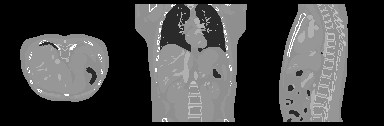
\includegraphics[width=0.9\textwidth]{Applications/XCAT.png} 
\end{center}

\caption[Cross section of the XCAT phantom]{\label{fig:XCAT} Cross section of the XCAT phantom in its mid plane in the three axes, for $128^3$ voxels.} 
\end{figure}

\begin{figure}[h]
\begin{center}

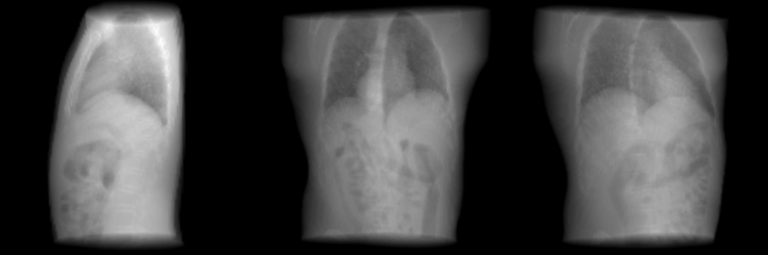
\includegraphics[width=0.9\textwidth]{Applications/XCATproj.png} 
\end{center}

\caption[Simulated projections of the XCAT phantom]{\label{fig:XCATproj} Simulate projections of the XCAT phantom at three different projection angles for a $256^2$ detector.} 
\end{figure}

\subsubsection{Update ordering in SART}

An analysis of the different ART-type algorithms is presented in this section. One of the discussed parameters that has an effect in the convergence rate of the ART-type algorithms is the ordering of the projections used. Research has shown that in ART, the angle ordering can have an effect on the residual\cite{herman1993algebraic}\cite{zouzias2013randomized}, however in the algorithms feasible for big scale tomography, this effect is smaller. Figure \ref{fig:SARTanglesconv} shows the convergence of SART during 150 iterations using 100 projections as data. The same configuration of SART is run using ordered, randomly ordered and angular distance maximizing ordering schemes for the update order. While minor, the figure shows how random ordering does generally increases the convergence rate of the algorithm, at no computational cost. This is the default value in the software. Note that in this test there is no reduction of the relaxation parameter $\lambda$.


\begin{figure}[H]
\begin{center}

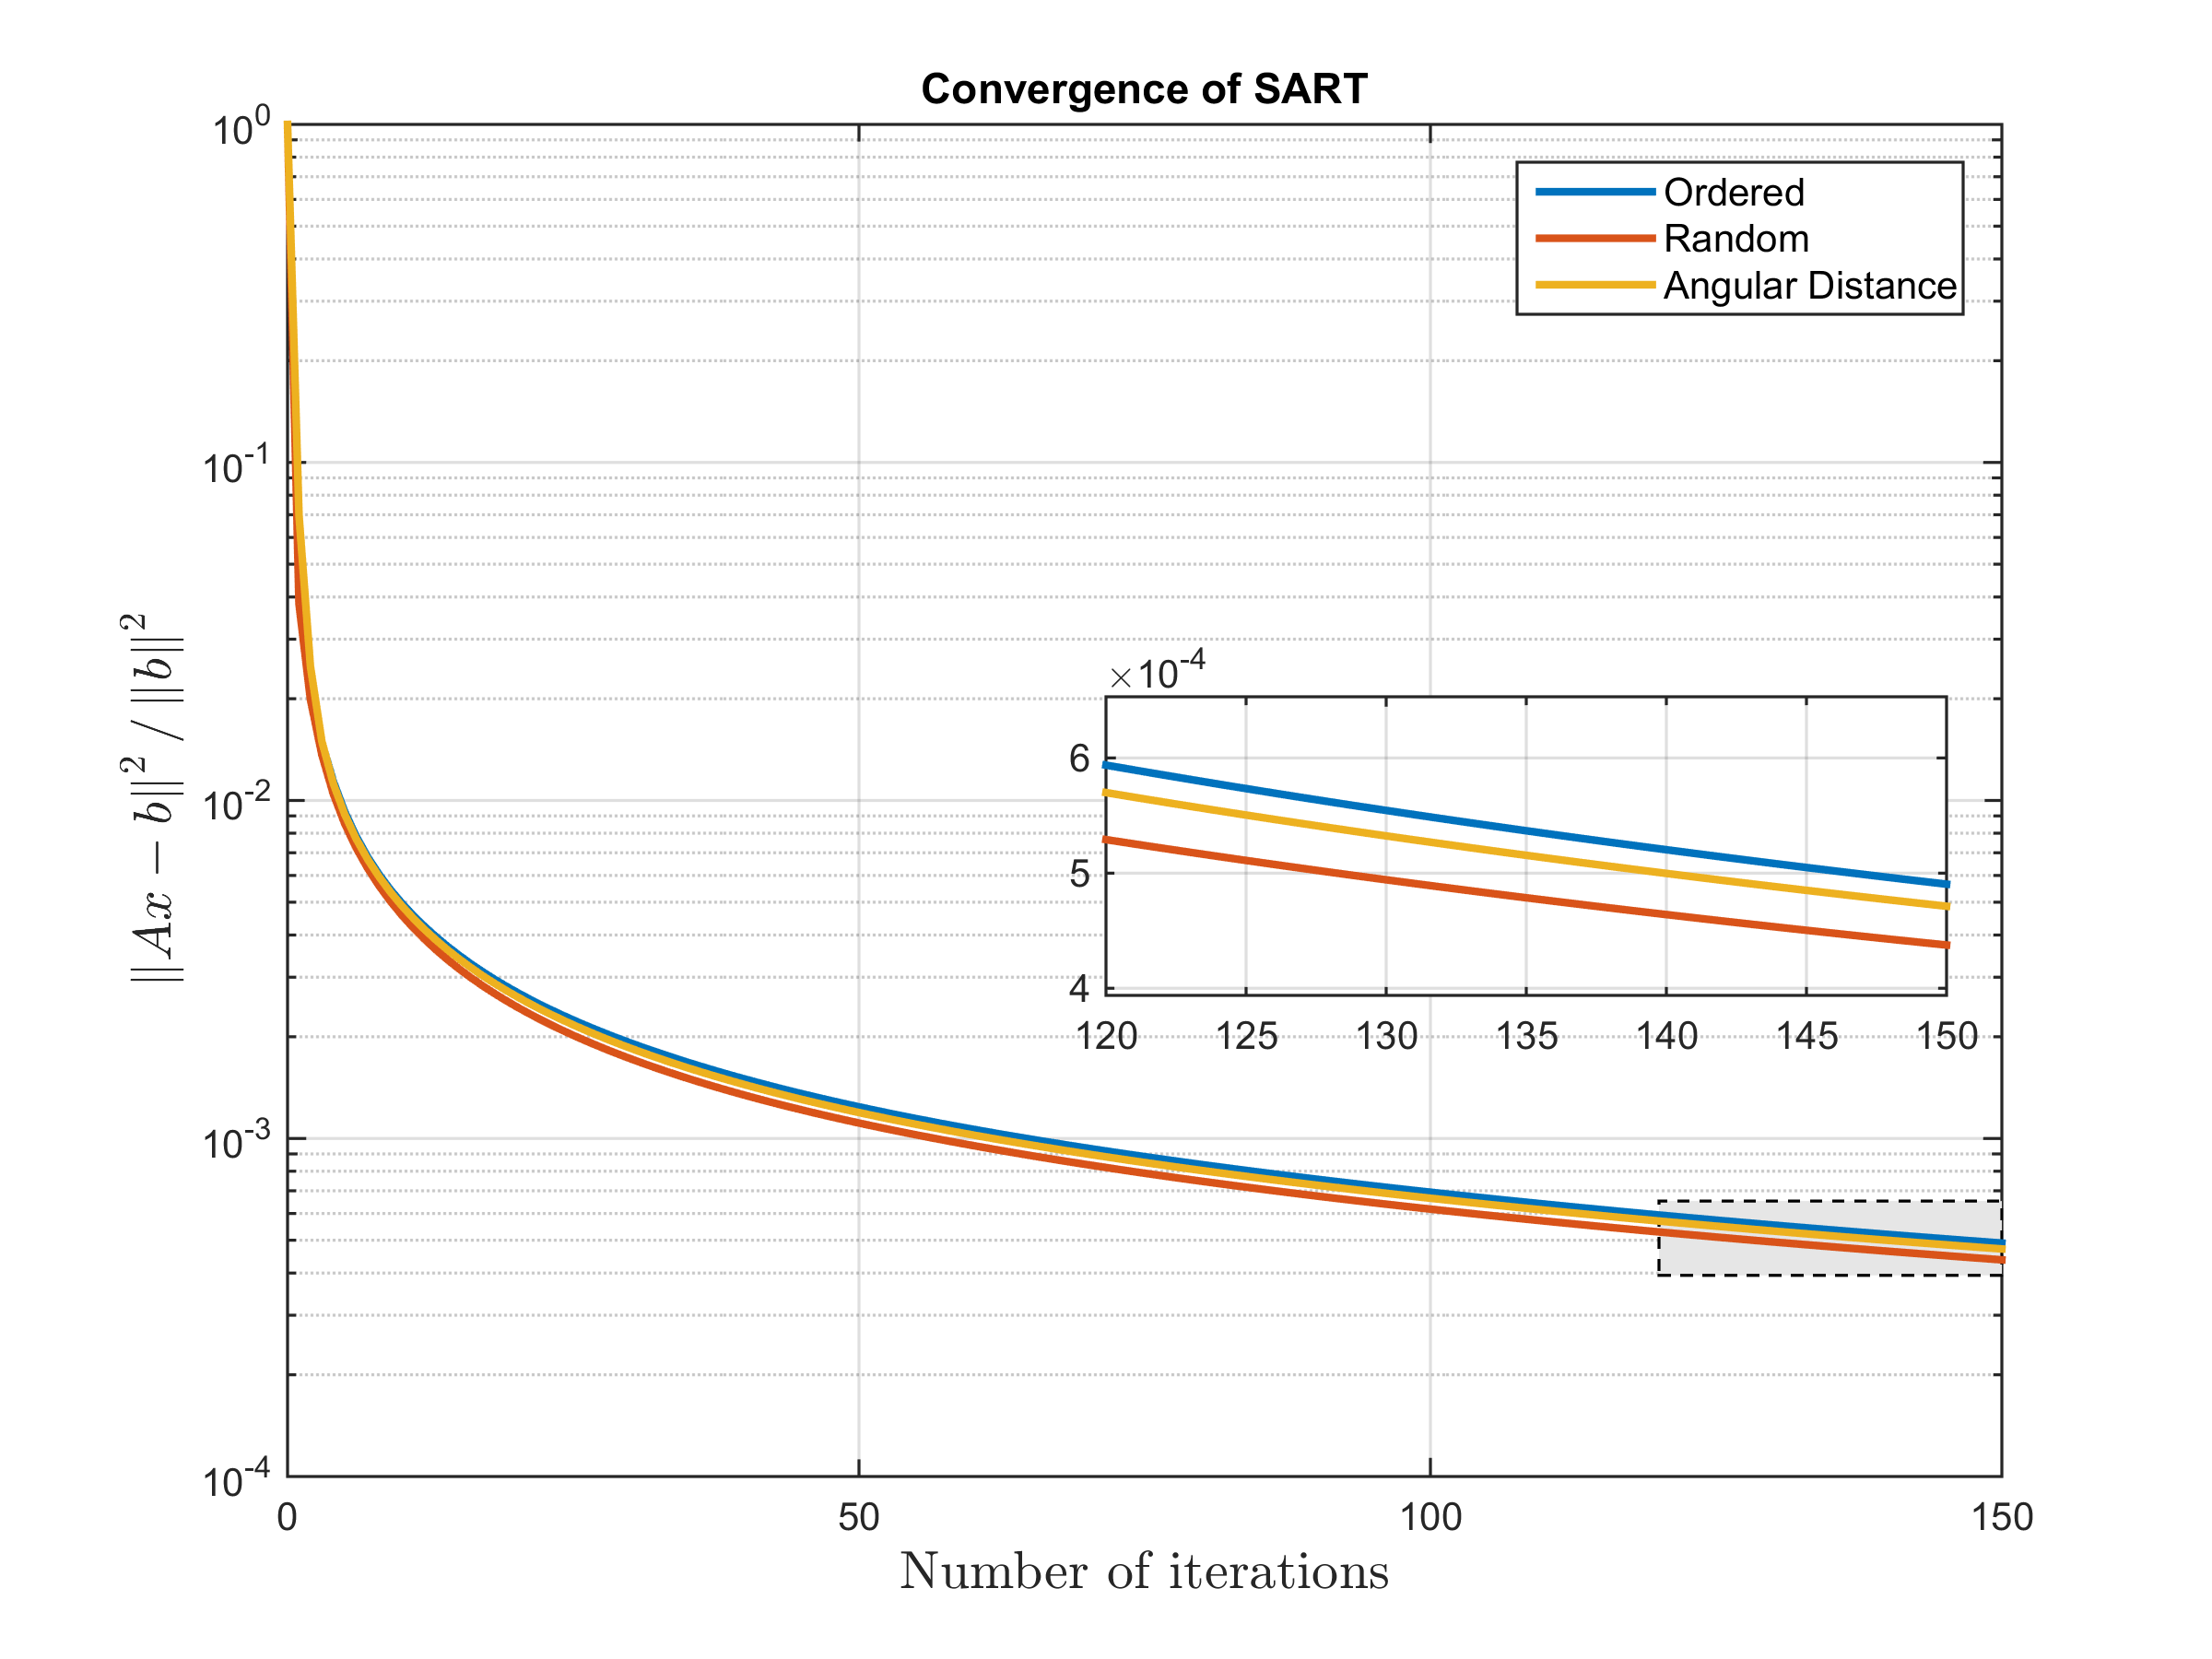
\includegraphics[width=0.8\textwidth]{Applications/SARTangles.png} 
\end{center}

\caption[Nomralized residual vs iteration of SART vs projection update order]{\label{fig:SARTanglesconv} Normalized residual versus iteration of SART compared to different angle ordering schemes, using 100 projections and no relaxation parameter reduction} 
\end{figure}

\subsubsection{Comparison between SART, OS-SART and SIRT}
These algorithms have very different convergence, as updating the image per-projection angle has the effect of converging faster (in iteration number). However, the computational times are greatly reduced by updating more rows at the same time. This effect can be seen in figure \ref{fig:SARTtypesconv}, where the convergence versus iteration of these three algorithms is plotted. Note the convergence difference between SART and SIRT, where SIRT doesn't reach SART's residual even after 1000 iterations, however, each iteration of SIRT is two orders of magnitude faster than SART. OS-SART provides a middle ground alternative. Due to the specifics of the acceleration procedures for backprojection, OS-SART speeds are closer to SIRT than to SART (i.e., the speed does not change linearly with the image updates per iteration), however it is more prone to divergent behaviour in TIGRE. In the figure, OS-SART stops converging after 48 iterations. Of course, this behaviour is very data-specific, and there are multiple cases where it does not diverge. Figure \ref{fig:SARTtypesconv} shows the result images of these three algorithms after 150 iterations (48 for OS-SART). Note that this example has limited data, so even in the best case, the images are slightly noisy.



\begin{figure}[H]
\begin{center}

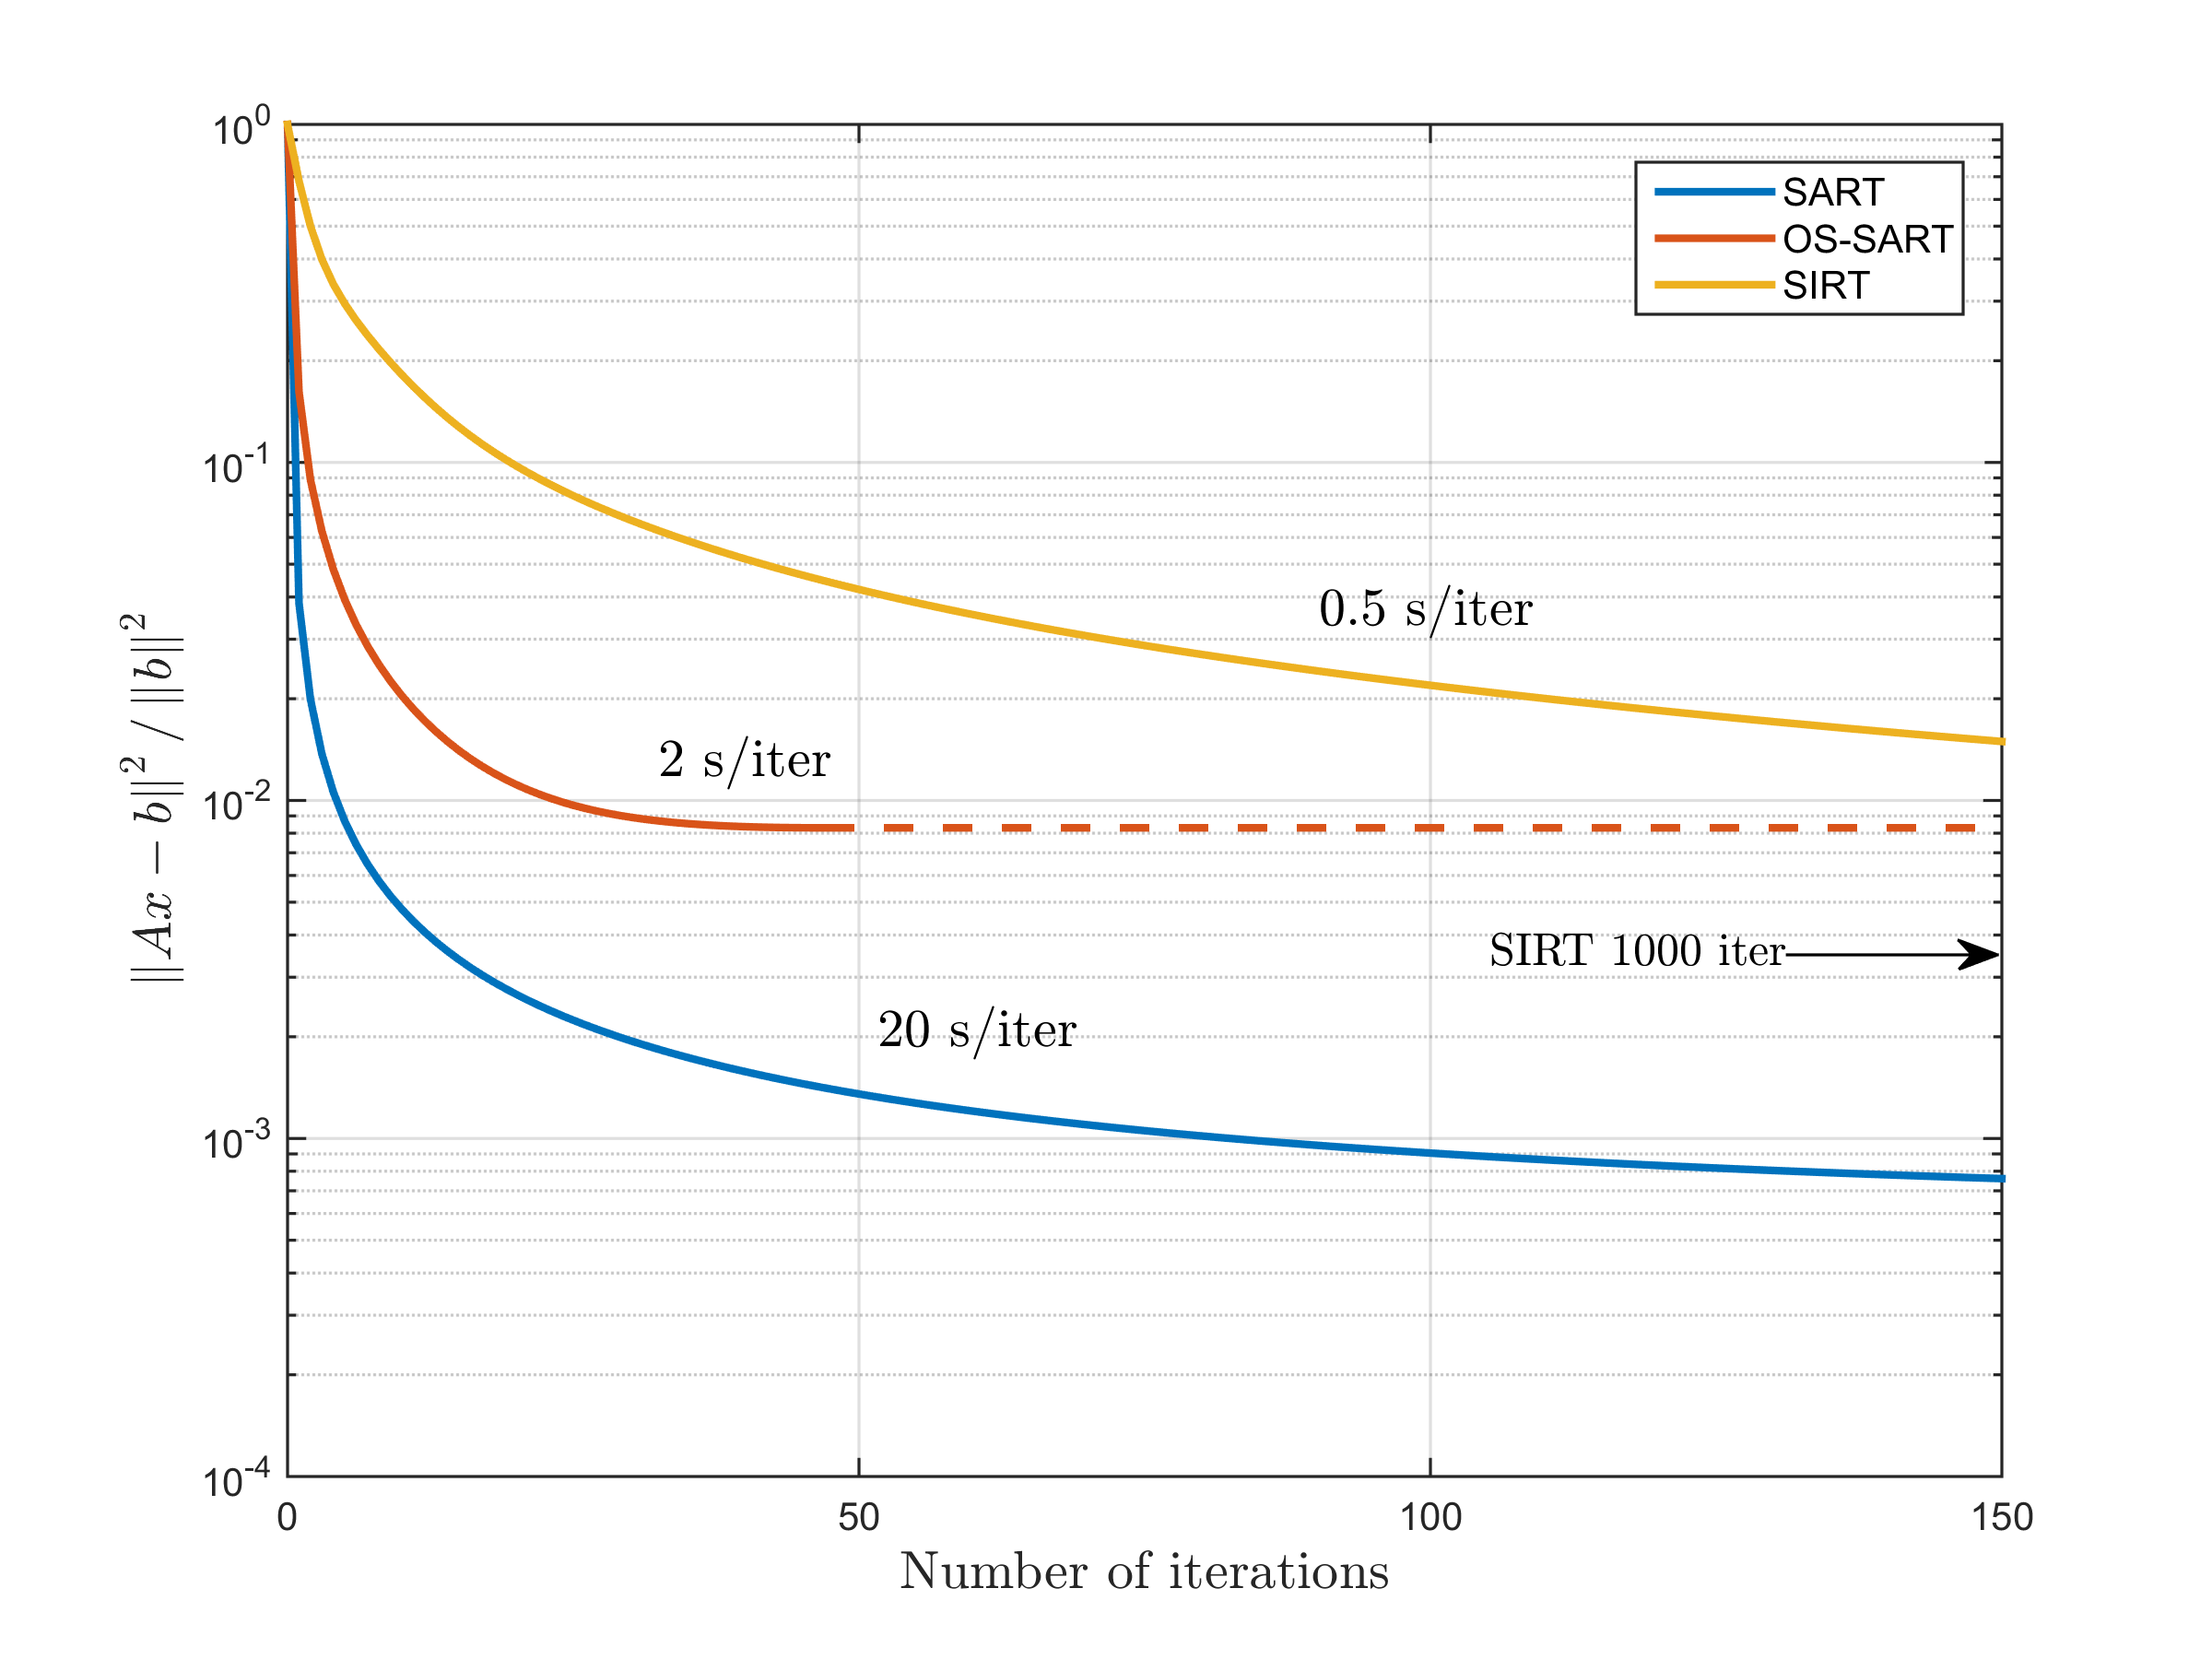
\includegraphics[width=0.8\textwidth]{Applications/SARTtypes.png} 
\end{center}

\caption[Nomralized residual vs iteration of SART/OS-SART/SIRT]{\label{fig:SARTtypesconv} Normalized residual vs iteration number for SART, OS-SART and SIRT using 100 projections and no relaxation parameter reduction.} 
\end{figure}

\subsubsection{Relaxation parameter}
The choice of a proper relaxation parameter significantly changes the speed which a solution is found, and can avoid infinitely iterating through the same hyperplanes in case of an under determined or noisy solution. In TIGRE, two methods are implemented, as described in Chapter 3: multiplying the relaxation parameter by a reduction factor after each iteration, and the Nesterov accelerated update, that does not technically update the relaxation parameter, but updates the image at each iteration using an iteration specific combination ratio of the gradients of the current and previous iterations. It requires more memory as it needs one extra image-sized variable to store the previous update, but the the algorithm finds a solution considerably faster, as can be seen in figure \ref{fig:SARTlambda}. In the figure each of the SART, OS-SART and SIRT algorithms residuals is plotted, and in each of them three versions are displayed, no relaxation parameter update, reduction with $r_{red}=0.99$ and the Nesterov update. In the plot it can also be seen that reducing the relaxation parameter by a ratio, while a good approach in SART-based hybrid algorithms such as the TV minimizing ones in TIGRE, leads to slower residual reduction and ultimately to a worse image.

In figure \ref{fig:SARTlambdaplot}, the solution found by the three algorithms using reduction of the relaxation parameter, using a Nesterov update and using a static relaxation parameter of $\lambda=1$ can be seen side by side. The superior solution found by Nesterov is clear, and both SART and OS-SART reach a minimum in very few iterations. While SART does reach a better image (both in residual and error) without using Nesterov's update, the difference is minimal. It is important to note that using Nesterov's update, likely due to its fast convergence, leads to a faster divergent behaviour by the algorithms, thus the residual needs to be checked in each iteration leading to some computational overhead.

\begin{figure}[H]
\begin{center}

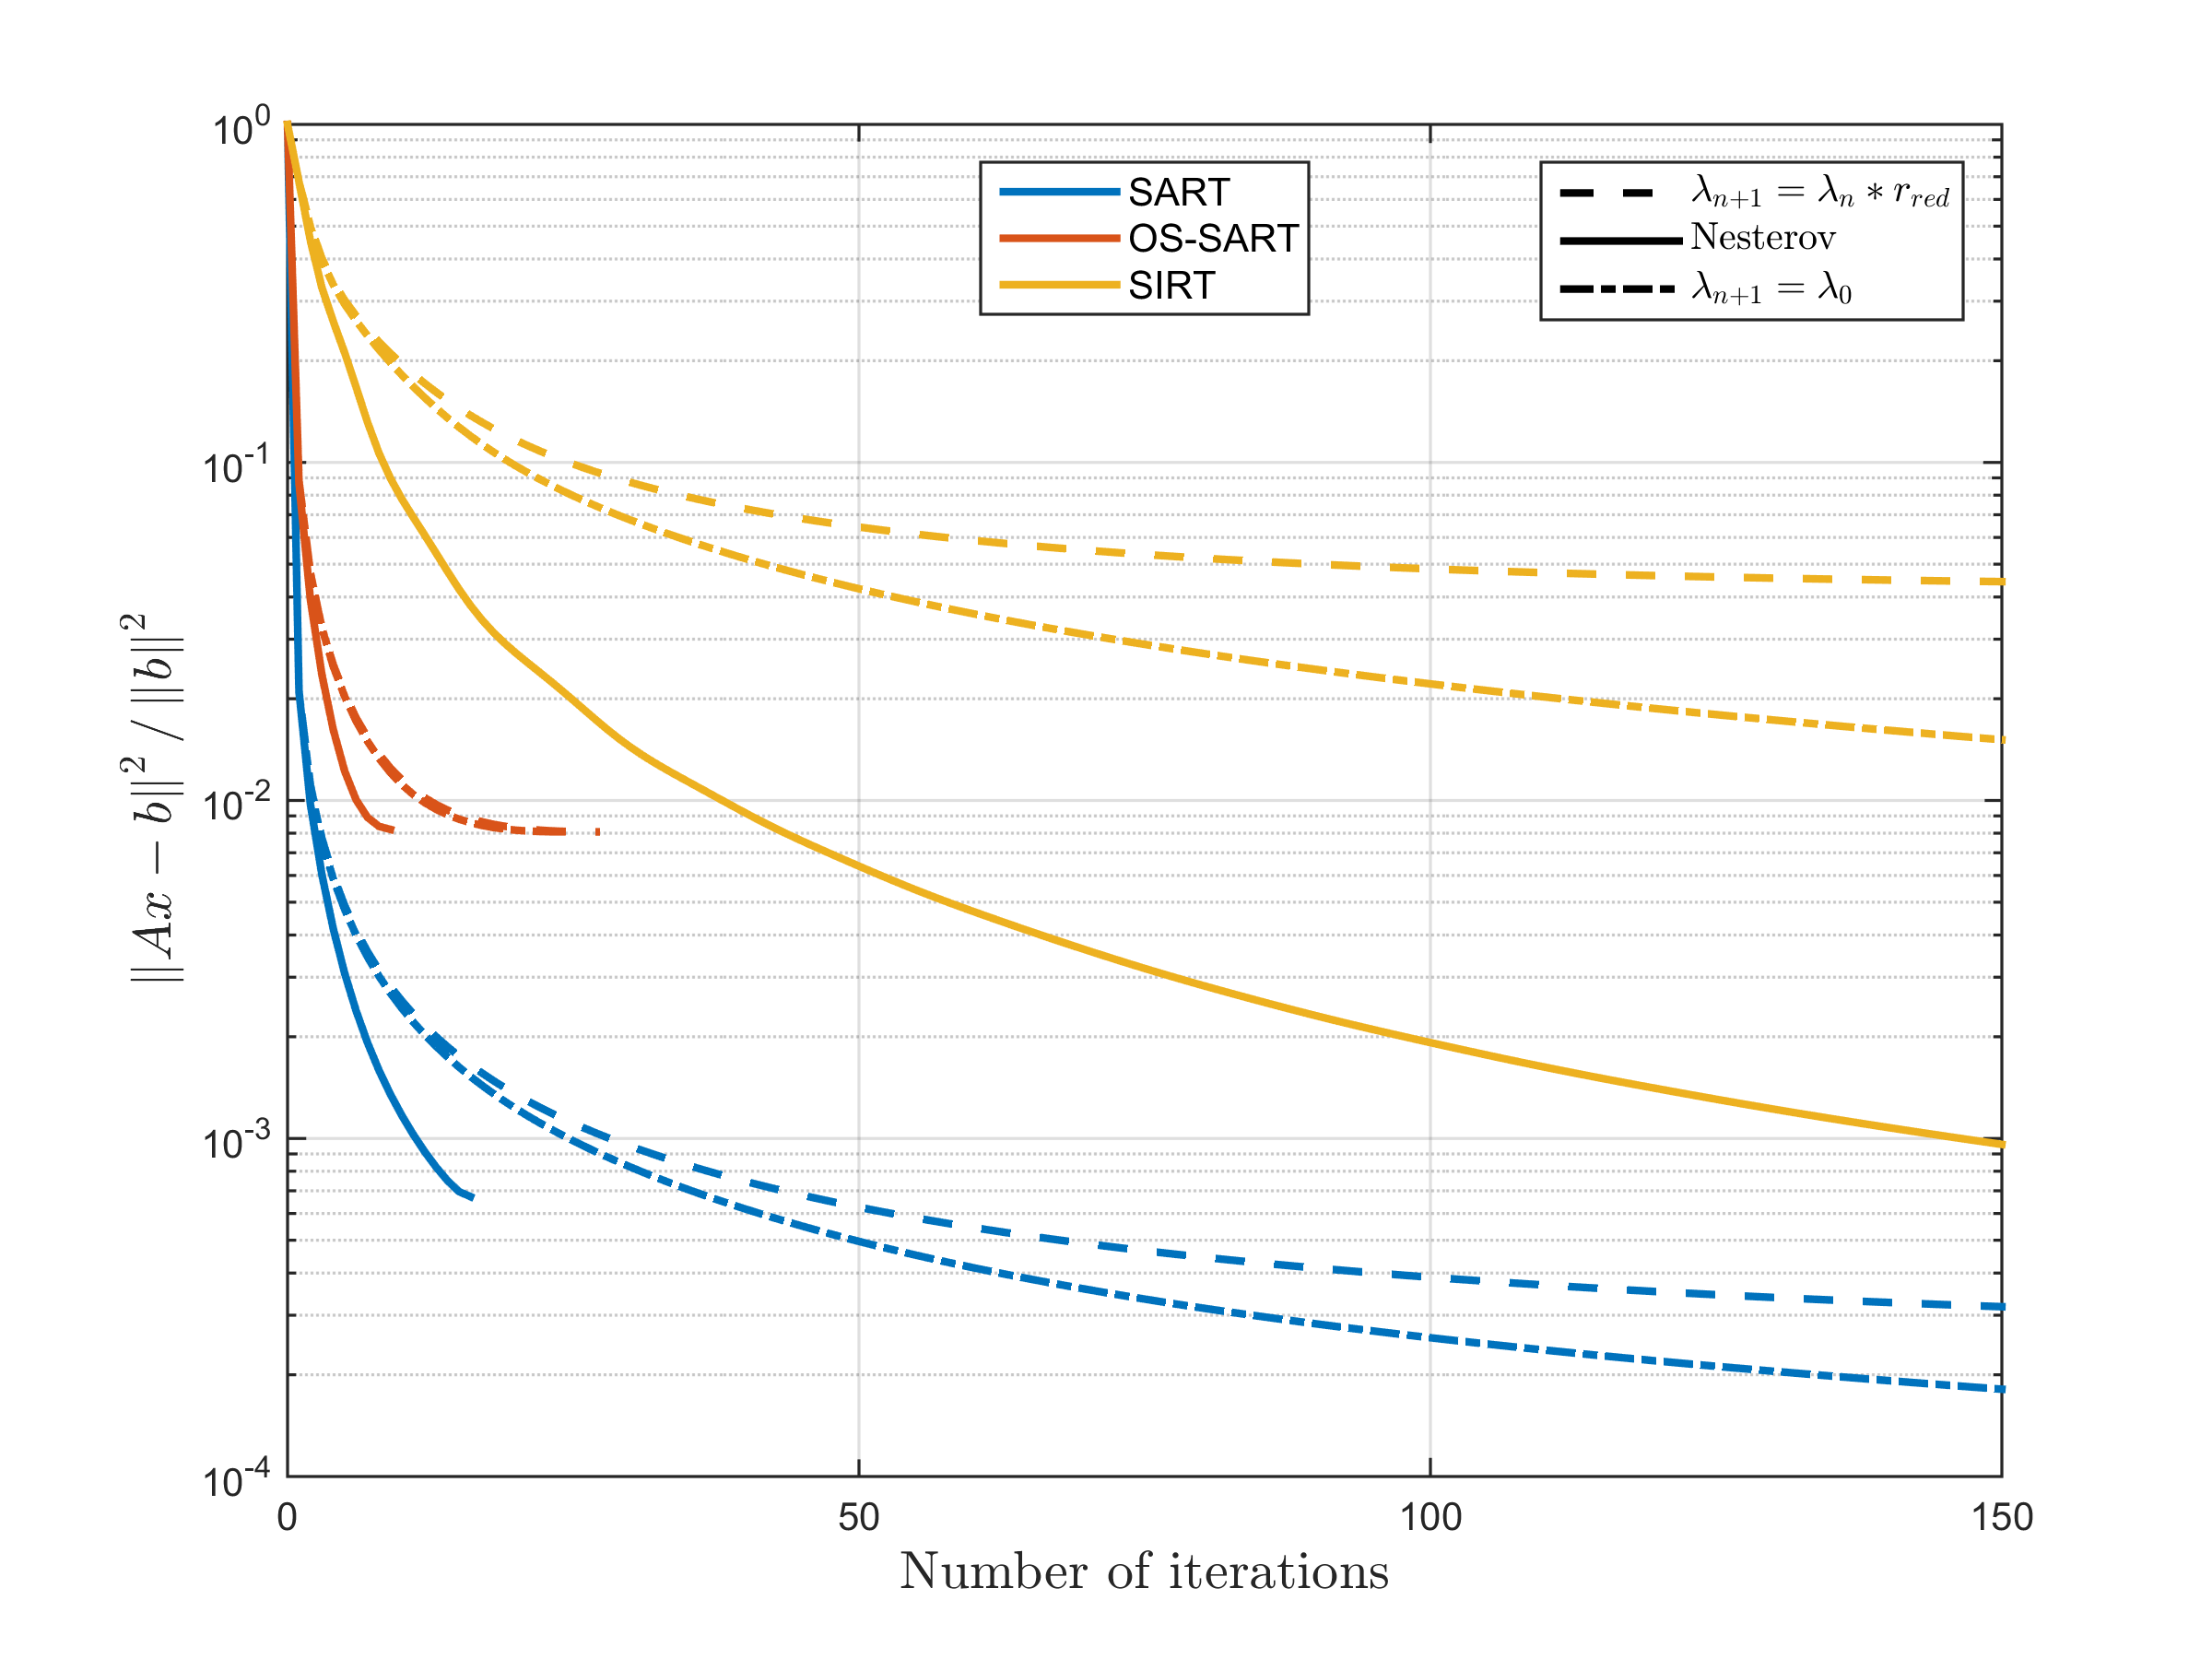
\includegraphics[width=0.8\textwidth]{Applications/SARTlambda.png} 
\end{center}

\caption[Nomralized residual vs iteration of SART/OS-SART/SIRT with different relaxation parameters]{\label{fig:SARTlambda} Normalized residual vs iteration number for SART, OS-SART and SIRT using 100 projections and different relaxation parameter reduction methods. If the relaxation parameter is reduced by a constant ratio, the residual reduction worsens, and if reduced using Nesterovs update, it converges very fast.} 
\end{figure}


\begin{figure}
\centering
\begin{tikzpicture}

\node (A) {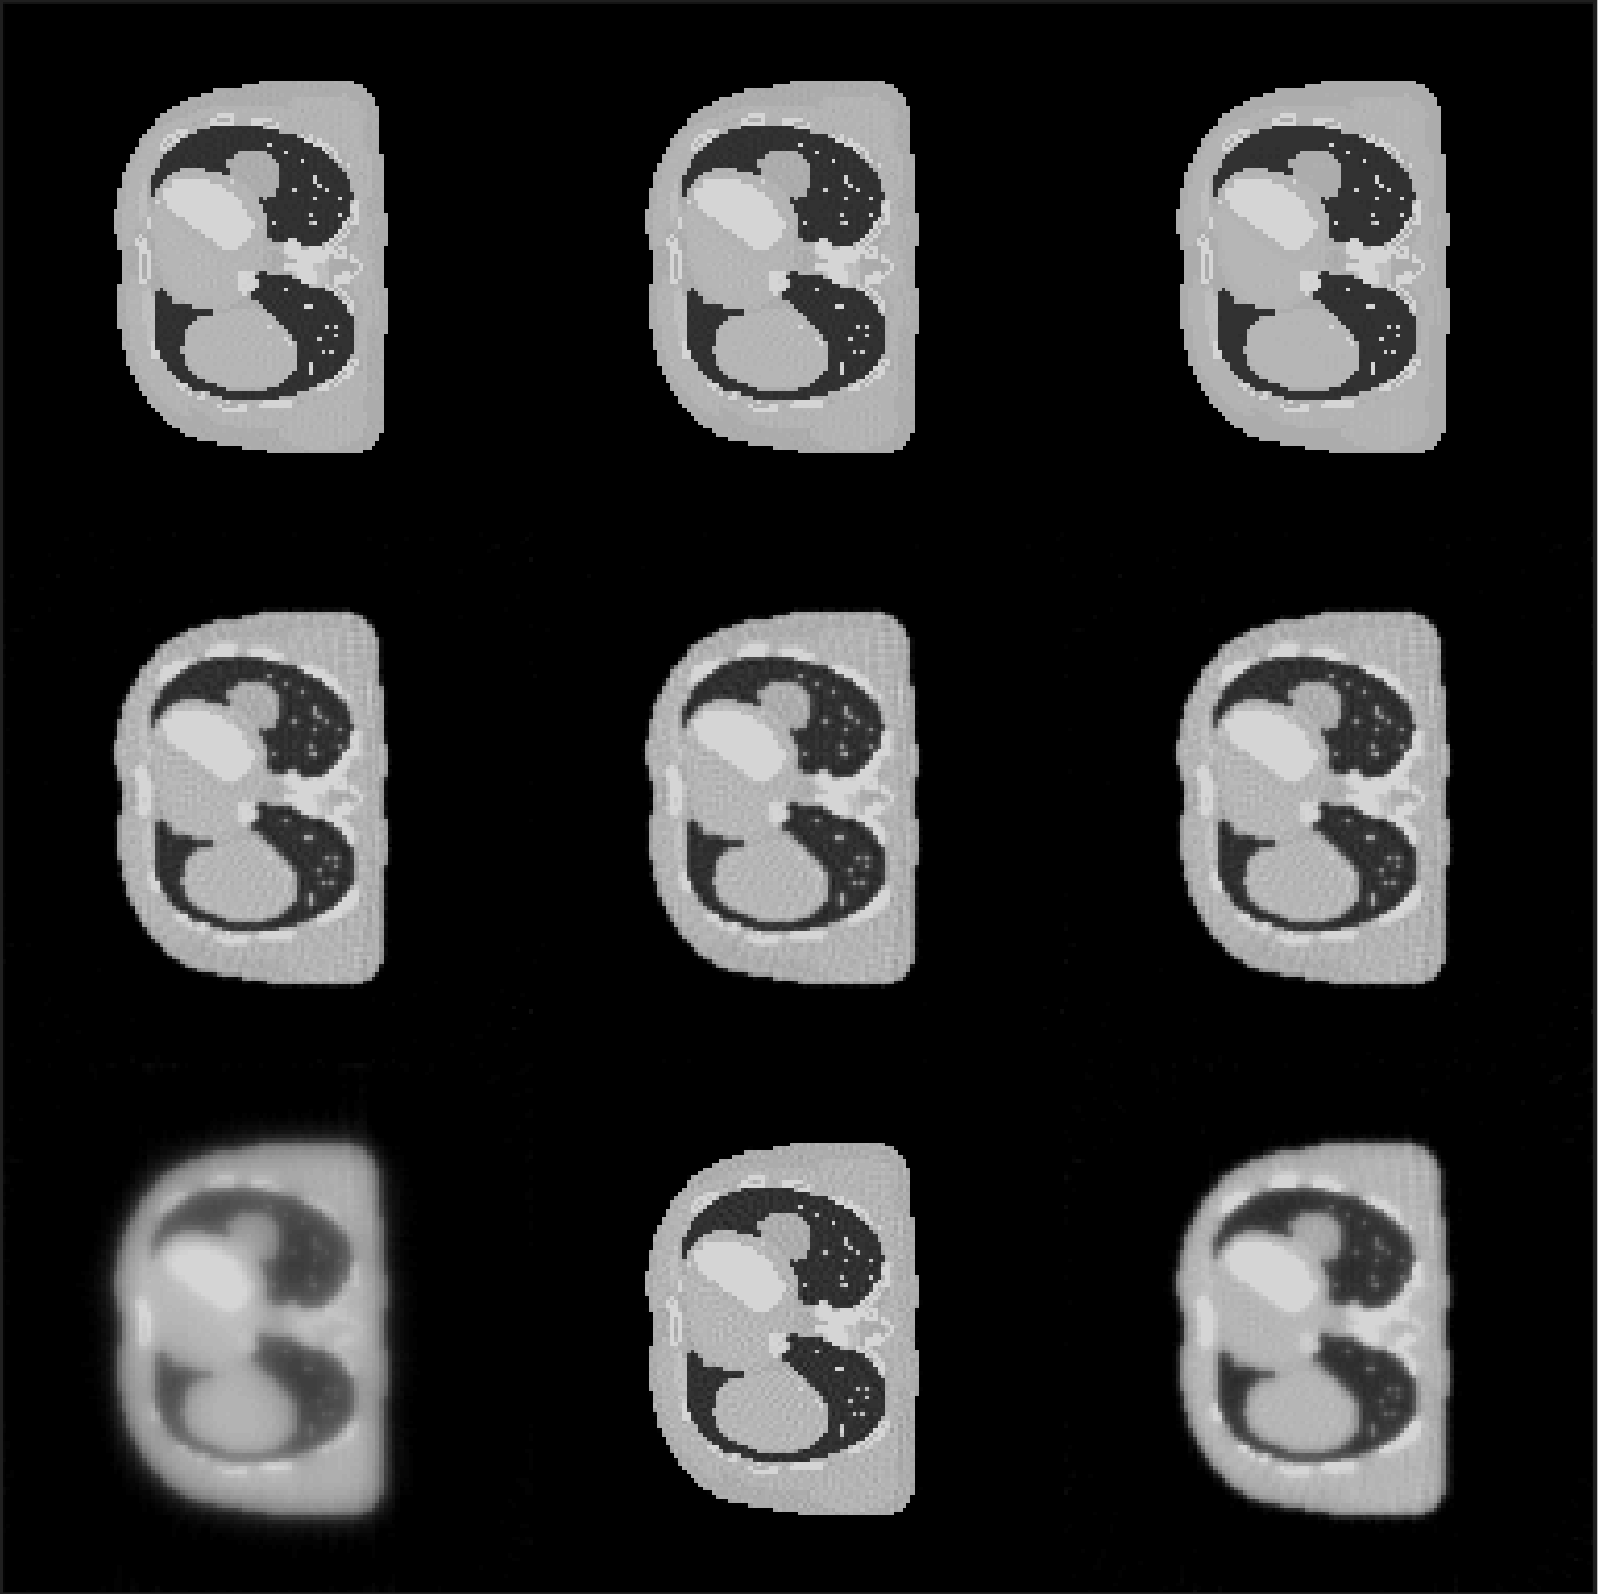
\includegraphics[width=0.94\textwidth]{Applications/SARTlambdaplot2.png} };
\path (A.south west) -- (A.north west) node[pos=.18, above, rotate=90] {SIRT} node[pos=.5, above, rotate=90] {OS-SART} node[pos=.82, above, rotate=90] {SART};
\path (A.south west) -- (A.south east) node[pos=.18, below] {$\lambda_{n+1}=\lambda_{n}r_{red}$} node[pos=.5, below] {Nesterov} node[pos=.82, below] {$\lambda_{n+1}=\lambda_0=1$};

\end{tikzpicture}
\caption[Reconstructed images with different relaxation parameter updates]{\label{fig:SARTlambdaplot}Reconstructed images with different relaxation parameter updates. OS-SART stops at iteration 24 in all but the Nesterov case, where it stops at iteration number 9. SART stops at iteration 16 for Nesterov.}
\end{figure}



\subsection{Total variation minimization}
There are four total variation minimizing algorithms in TIGRE, with 2 different minimization functionals. As previously described, ASD-POCS, OS-ASD-POCS and B-ASD-POCS-$\beta$ minimize the TV using a POCS minimization technique by minimizing the data constraint and TV norm independently using gradient descent. SART-TV however uses the ROF model for the TV-minimization step. The total variation algorithms are designed for applications where the image is piecewise-smooth, as they will try to minimize the gradient, by creating single-valued regions in the image. In CT, the most noisy images are reconstructed when either the data is very noisy (generally due to small acquisition times and/or low energy X-rays) or when the data are limited, either due to limited angular range or more importantly a limited number of projections. 

An example of the behaviour of the TV algorithms with the same dataset as in figures \ref{fig:XCAT} and \ref{fig:XCATproj} is shown in figure \ref{fig:TVXCAT}. In this case, 30 uniformly sampled projections are used perturbed with Poisson and Gaussian noise to simulate photon scattering and electronic noise, respectively. The figure shows FDK and OS-SART reconstructions, and the four mentioned TV algorithms. It is clear that the TV algorithms do provide a smoother reconstruction, and with less normalized root mean squared error (NRMSE), as shown in table \ref{tab:NRMSE TVs}.
The reconstruction by FDk is plagued with noise. And, while the main structural features can be seen, most of the detail is lost. Even the bones themselves are practically indistinguishable from noise. OS-SART does reconstruct a smoother image as expected, as it minimizes the 2-norm and, while one can see more details in the image, it is still poor. The four TV algorithms can be seen to flatten out the attenuation levels to similar values, thus reducing most of the noise. Additionally most of the features get clearly separated from the attenuation levels of the surrounding tissues and some of the algorithms (such as ASD-POCS) are able to reconstruct even single pixel width structures correctly. It is important to note that while the parameters used to tune this specific TV reconstruction (available in demo number 9 in the TIGRE Toolbox), they are far from optimal and very sensitive\cite{Vee}. When choosing the exact optimal parameters for the TV reconstruction algorithms, the resultant images tend to be significantly better than the ones shown here, but the parameter space is very data dependent and large, thus to the author's knowledge, no parameter selection method has been proposed in the literature. 


\begin{figure}
\centering
\begin{tikzpicture}

\node (A) {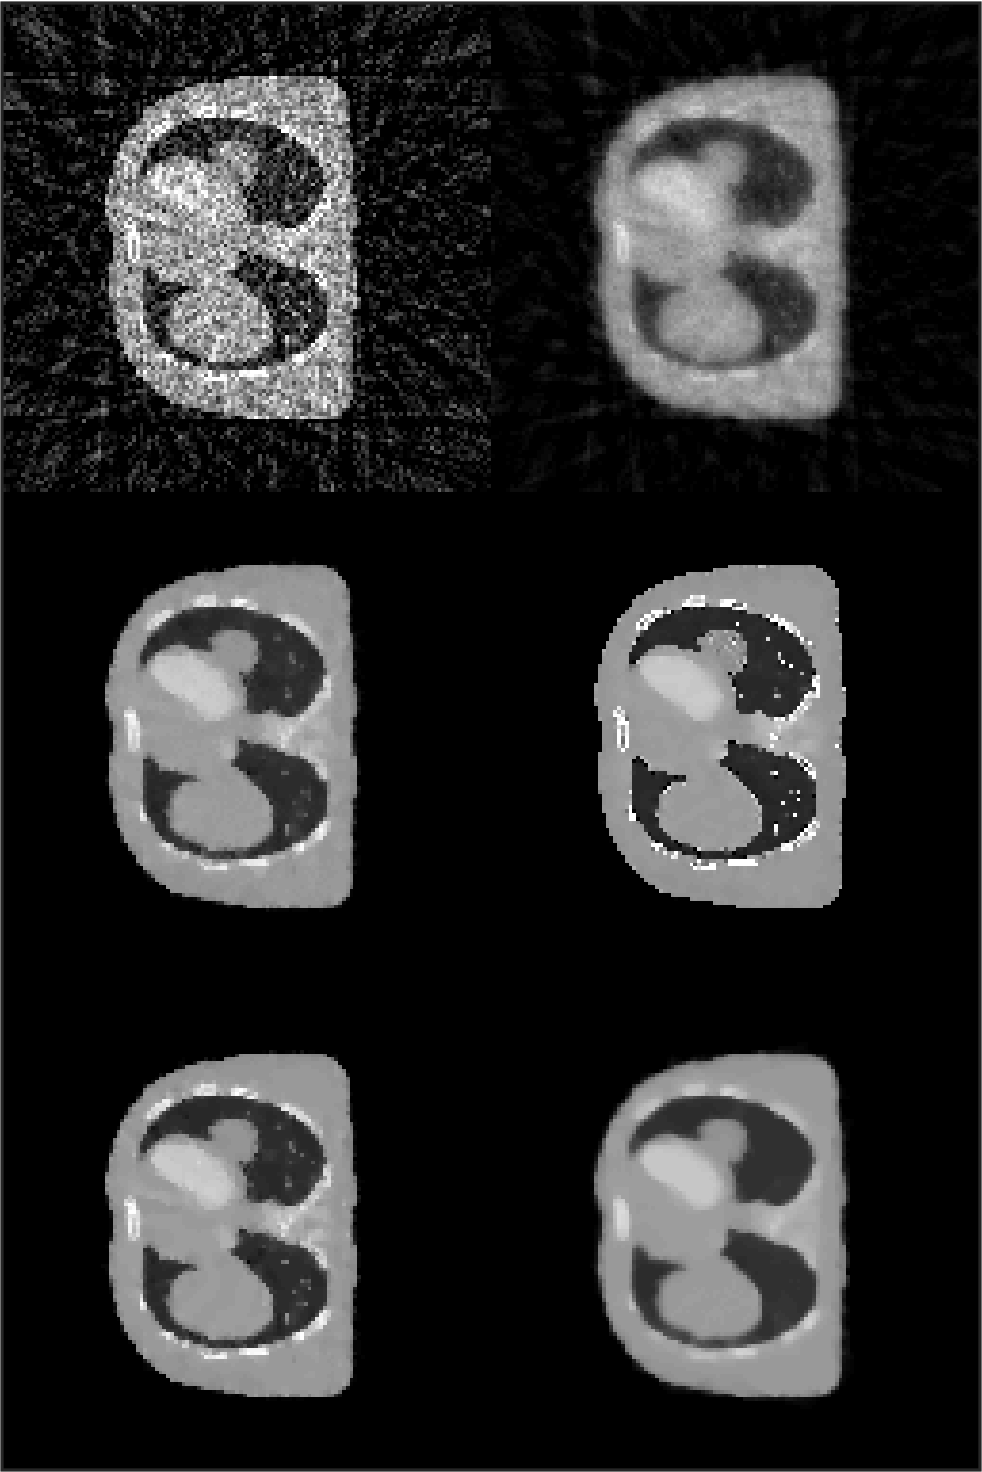
\includegraphics[width=0.4\textwidth]{Applications/TVs.png} };
\path (A.south west) -- (A.north west) node[pos=.18, above, rotate=90] {ASD-POCS} node[pos=.5, above, rotate=90] {B-ASD-POCS-$\beta$} node[pos=.82, above, rotate=90] {FDK};
\path (A.south east) -- (A.north east) node[pos=.18, below, rotate=90] {OS-ASD-POCS} node[pos=.5, below, rotate=90] {SART-TV} node[pos=.82, below, rotate=90] {OS-SART};

\node (B)at (0.5\textwidth,0) {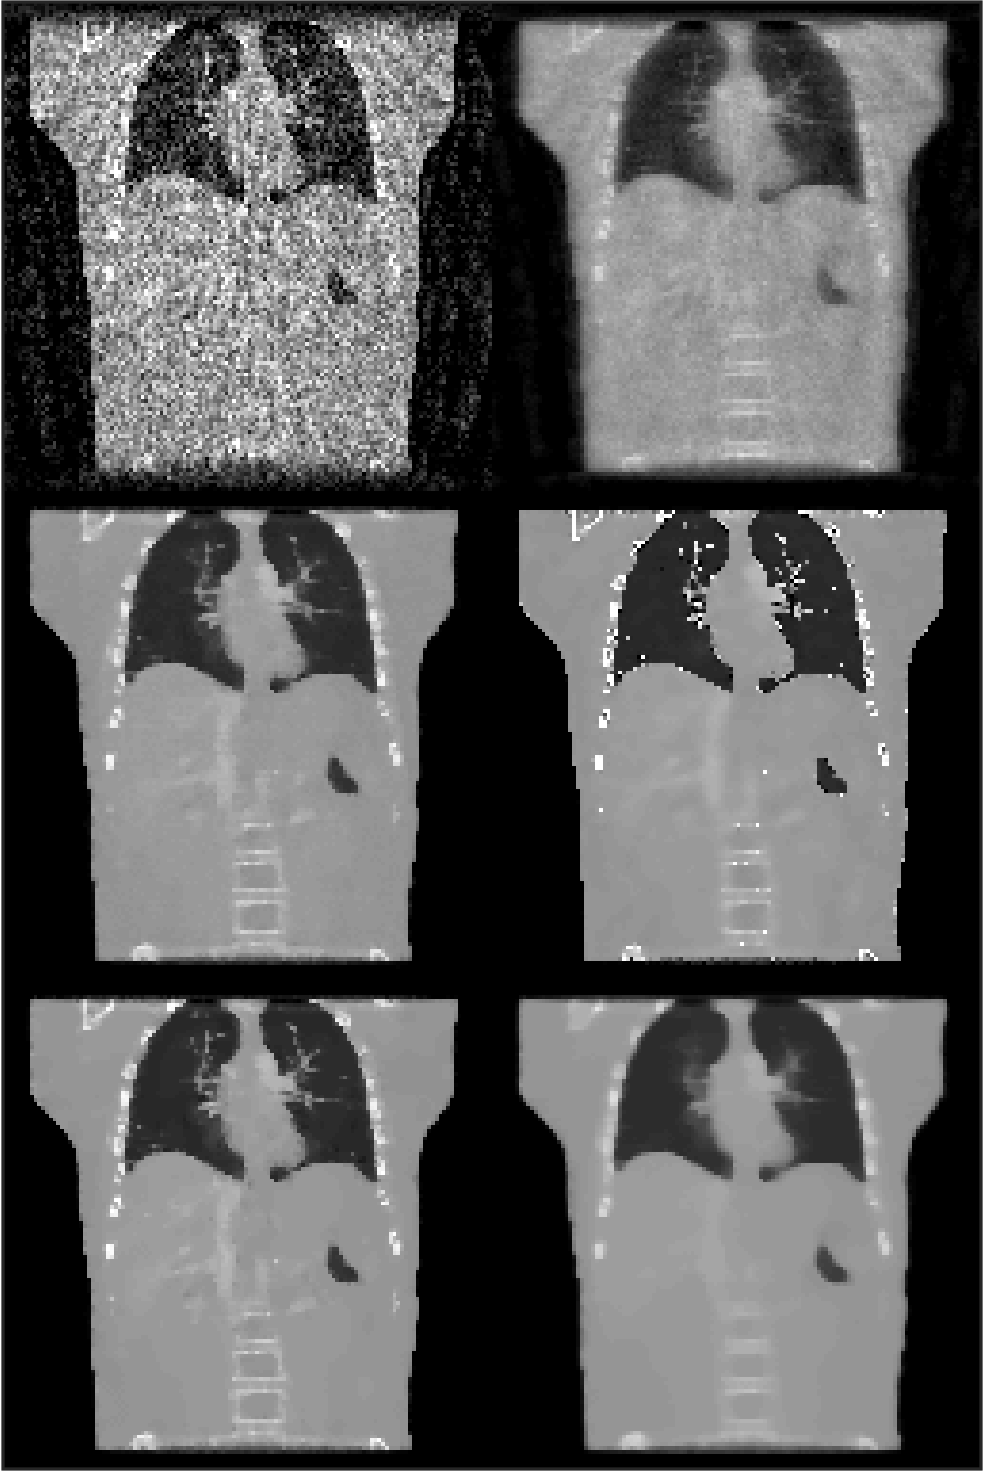
\includegraphics[width=0.4\textwidth]{Applications/TVs2.png} };
\path (B.south west) -- (B.north west) node[pos=.18, above, rotate=90] {ASD-POCS} node[pos=.5, above, rotate=90] {b-ASD-POCS-$\beta$} node[pos=.82, above, rotate=90] {FDK};
\path (B.south east) -- (B.north east) node[pos=.18, below, rotate=90] {OS-ASD-POCS} node[pos=.5, below, rotate=90] {SART-TV} node[pos=.82, below, rotate=90] {OS-SART};

\end{tikzpicture}
\caption[Reconstructed images using TV algorithms]{\label{fig:TVXCAT}Reconstructed images using FDK, OS-SART and the TV algorithms b-ASD-POCS-$\beta$, SART-TV,  ASD-POCS and OS-ASD-POCS with a limited amount and noisy data. Both figures show the same data and algorithms, but with a different cross-section of the image.}
\end{figure}


\begin{table}
\begin{center}
\caption{NRMSE for the reconstructed images in figure \ref{fig:TVXCAT}}
\label{tab:NRMSE TVs}
\scalebox{0.85}{
\begin{tabular}{| l || c | c | c | c | c | c |}
\hline
& FDK & OS-SART &B-ASD-POCS-$\beta$&SART-TV& ASD-POCS& OS-ASD-POCS\\  
\hline
\hline
NRMSE&  0.1373  &  0.0678  &  0.0338   & 0.0267 &   0.0304 &   0.0442\\   

\hline  
\end{tabular}
}
\end{center}
\end{table}






To illustrate the sensitivity to parameter selection, the algorithm SART-TV is run with three different values for the number of TV-iterations per SART iteration for the same data set used in the previous test. The results can be seen in figure \ref{fig:SARTTVparams}, where one can clearly see how small changes can have a devastating effect in the output image.   If a few more TV iterations are added to (b), the image gets a bit smoother and some detail is lost, as expected. However, if few iterations are removed from (b), the image can get completely destroyed. Note that these values are only applicable to this image with the exact amount of noise and projections. Different experiments may not show this behaviour or may be more intolerant to parameter change. This is arguably the biggest limitation for the common use of TV algorithms in real applications. As an advantageous point, once the good parameters are found, generally the algorithm will perform similarly for similar images, thus application specific parameters may be an option.






\begin{figure}
\centering
\begin{tikzpicture}

\node (A) {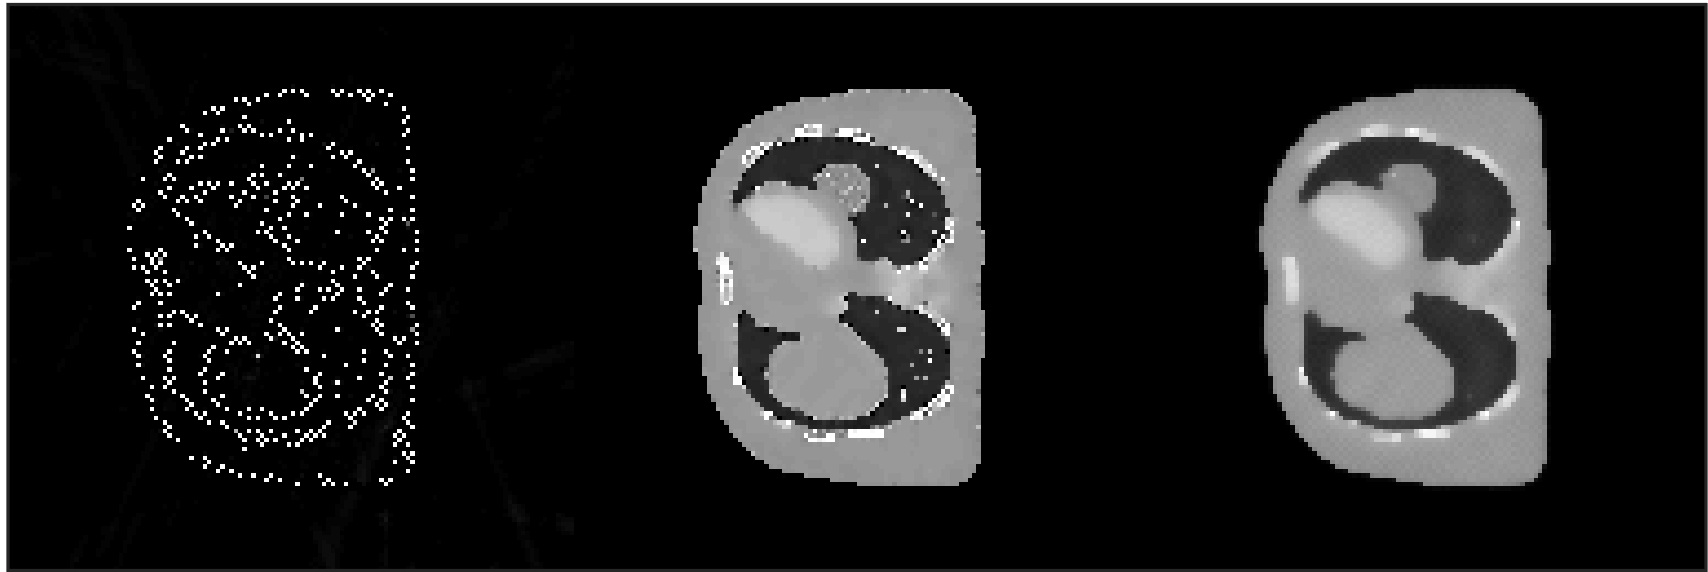
\includegraphics[width=0.7\textwidth]{Applications/TVs3.png} };
%\path (A.south west) -- (A.north west) node[pos=.18, above, rotate=90] {ASD-POCS} node[pos=.5, above, rotate=90] {b-ASD-POCS-$\beta$} node[pos=.82, above, rotate=90] {FDK};
\path (A.south west) -- (A.south east) node[pos=.18, below] {(a)} node[pos=.5, below] {(b)} node[pos=.82, below] {(c)};

\end{tikzpicture}
\caption[SART-TV algorithms with different parameters]{\label{fig:SARTTVparams}SART-TV algorithms with different amount of TV iterations per SART iteration, (a) 32 iterations, (b) 40 iterations, (c) 48 iterations.}
\end{figure}



\FloatBarrier
\section{Iterative algorithms in different CT applications}
This section tries to illustrate the effect of different algorithms within the TIGRE Toolbox for a series of datasets. 
\subsection{Medical head CBCT from  The Christie Hospital}

This dataset is a RANDO head phantom that represents a head of an adult. The dataset was acquired in The Christie Hospital in Manchester, and consists of 360 equiangular projections over a full rotation. The dataset has mechanical offsets and high noise, as it has been tuned to work for head CBCT, so its low intensity X-rays (exact parameters not known). In this test, the sample has been reconstructed using FDK, CGLS, OS-SART and OS-ASD-POCS (ASD-POCS with OS-SART instead of SART for the data constraint). Figure \ref{fig:RANDO360} shows the reconstruction using 360 angles, while figure \ref{fig:RANDO90} shows the reconstruction using 90 angles. While in all algorithms the quality is worse when reducing the amount of data, most features are clear in the iterative algorithms with 90 projections, while some are a slightly obscured in the low exultation FDK, specially the thin bone walls.

\begin{figure}
\begin{center}
\begin{tikzpicture}

\node (A) {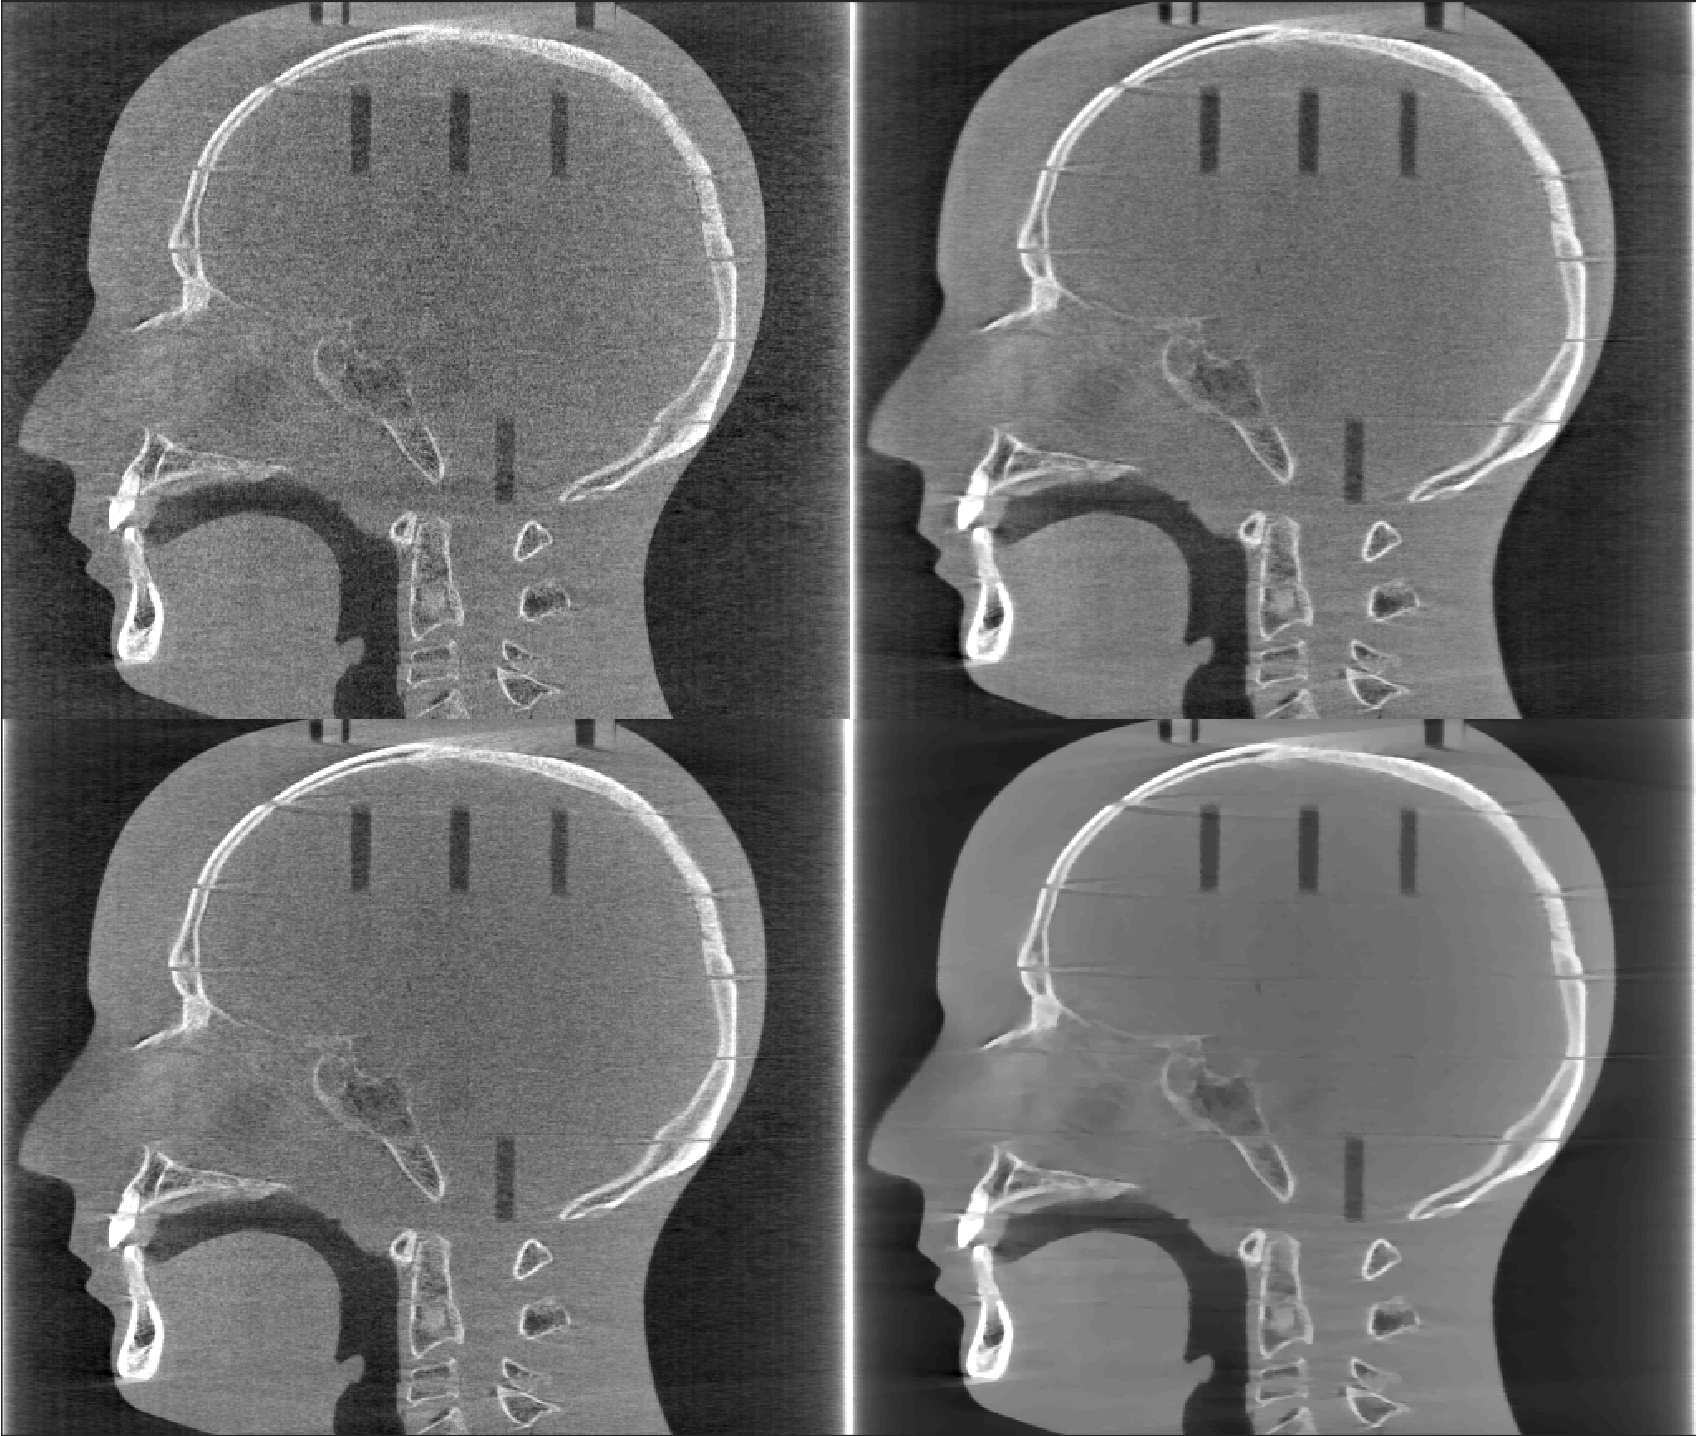
\includegraphics[width=0.4\textheight]{Applications/randofull.png}  };
\path (A.south west) -- (A.north west) node[pos=.25, above, rotate=90] {OS-SART} node[pos=.75, above, rotate=90] {FDK};
\path (A.south east) -- (A.north east) node[pos=.25, below, rotate=90] {OS-ASD-POCS} node[pos=.75, below, rotate=90] {CGLS} ;

\end{tikzpicture}

\end{center}

\caption[RANDO head using 360 projections and 4 algorithms]{\label{fig:RANDO360} RANDO head using 360 equiangular projections, with 4 different algorithms, FDK, CGLS, OS-SART and OS-ASD-POCS. The displaying window is [0-0.05]} 
\end{figure}
\begin{figure}
\begin{center}
\begin{tikzpicture}

\node (A) {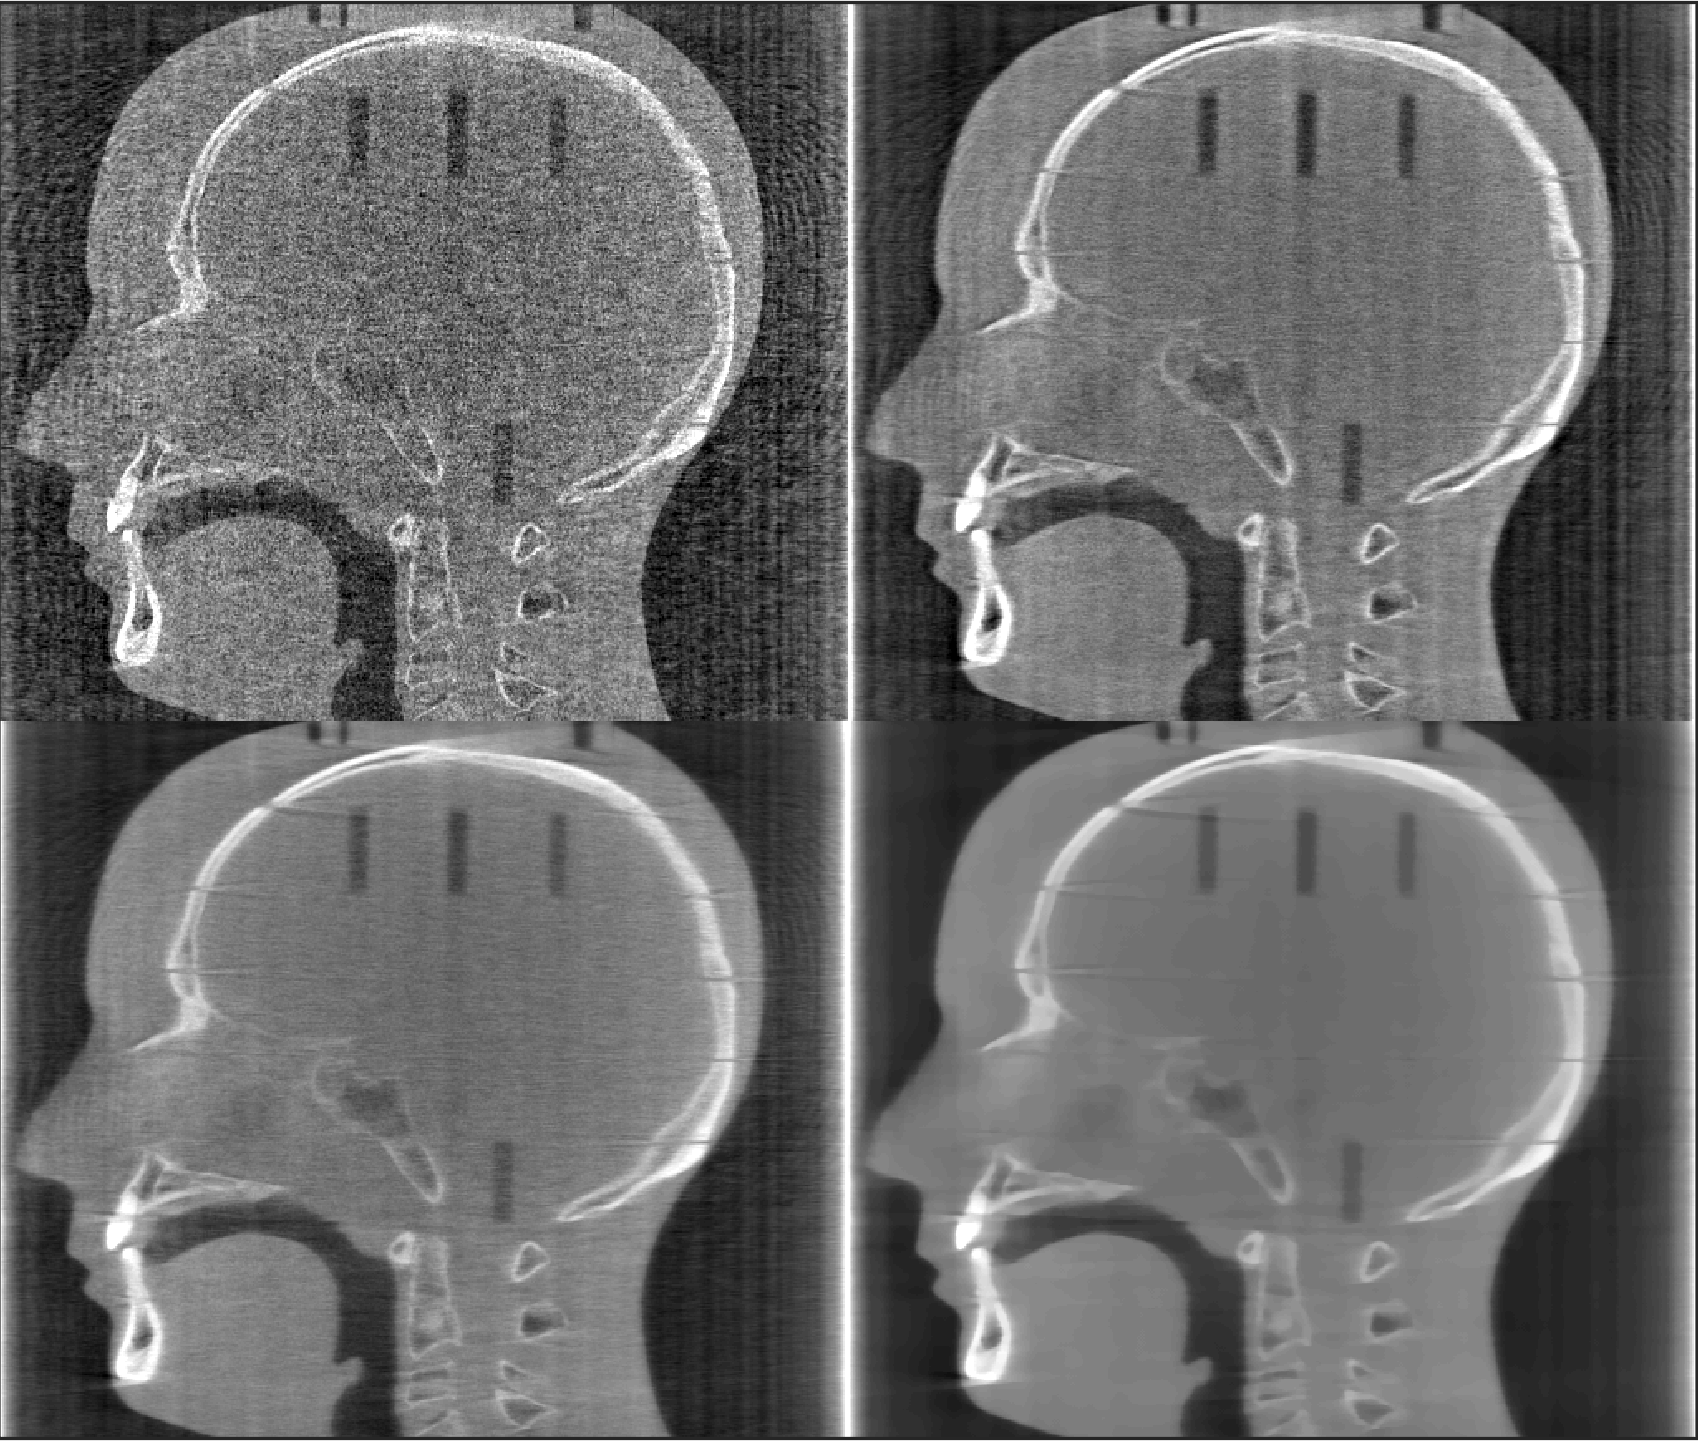
\includegraphics[width=0.4\textheight]{Applications/rando90.png}  };
\path (A.south west) -- (A.north west) node[pos=.25, above, rotate=90] {OS-SART} node[pos=.75, above, rotate=90] {FDK};
\path (A.south east) -- (A.north east) node[pos=.25, below, rotate=90] {OS-ASD-POCS} node[pos=.75, below, rotate=90] {CGLS} ;

\end{tikzpicture}

\end{center}

\caption[RANDO head using 90 projections and 4 algorithms]{\label{fig:RANDO90} RANDO head using 90 equiangular projections, with 4 different algorithms, FDK, CGLS, OS-SART and OS-ASD-POCS. The displaying window is [0-0.05]} 
\end{figure}

\FloatBarrier

\subsection{Micro-tomography: SophiaBeads dataset}
Another widespread application of tomography is industrial tomography,and specifically micro-tomography, for inspecting pieces from manufacturing processes. A dataset presented for testing algorithms in these conditions was published by Sophia \textit{et al}\cite{coban_2015_16539}\cite{coban2015sophiabeads} that has a pile of beads in a tube. The description of the data from their webpage\cite{coban_2015_16474} reads: ``SophiaBeads Dataset are acquired specifically for testing and comparing reconstruction methods for X-ray computed tomography. The sample is a plastic tube with a diameter of 25 mm, filled with uniform Soda-Lime Glass (SiO2-Na2O) beads of diameters 2.5 mm (with standard deviation 0.1 mm)''. The dataset containing 256 projections has been reconstructed in a 500$\times$500$\times$200 voxels image using FDK and CGLS, and the reconstructed images can be seen in figure \ref{fig:sophia1}. The red line shows a profile path that is shown for both FDK and CGLS in figure \ref{fig:sophiaprofile}. \tb{There are various things that would suggest that CGLS reconstructs a better image. The FDK image can be seen to have higher noise in the profile. The FDK image too, generates a high amount of streak artefacts in the empty surrounding area, while the CGLS suppresses this clearly, showing a relatively plalin background. Similarly, the uniformity of the attenuation coefficient is quite high in the CGLS reconstruction compared to the FDK reconstruction, where random peaks can be seen all around. Overall The CGLS image shows boundaries of the objects with the same accuracy as FDK, plus does not add (or perhaps suppresses) noise.}

\begin{figure}
\begin{center}

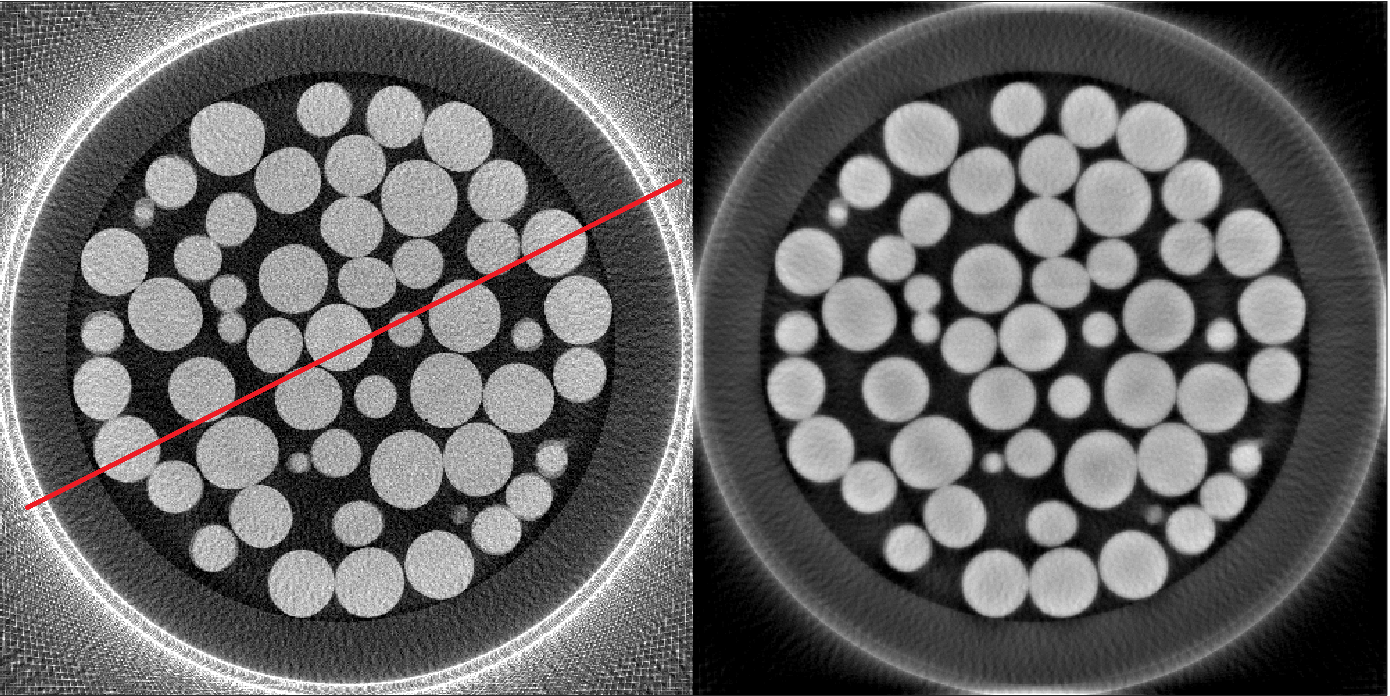
\includegraphics[width=\textwidth]{Applications/sophiaFDKCGLS.png} 

\end{center}

\caption[SophiaBeads dataset with FDK and CGLS]{\label{fig:sophia1} SophiaBeads dataset with FDK and CGLS (15 iterations), using 256 projections. The red line shows the profile evaluated. The display window is [0-0.15]. } 
\end{figure}
\begin{figure}
\begin{center}

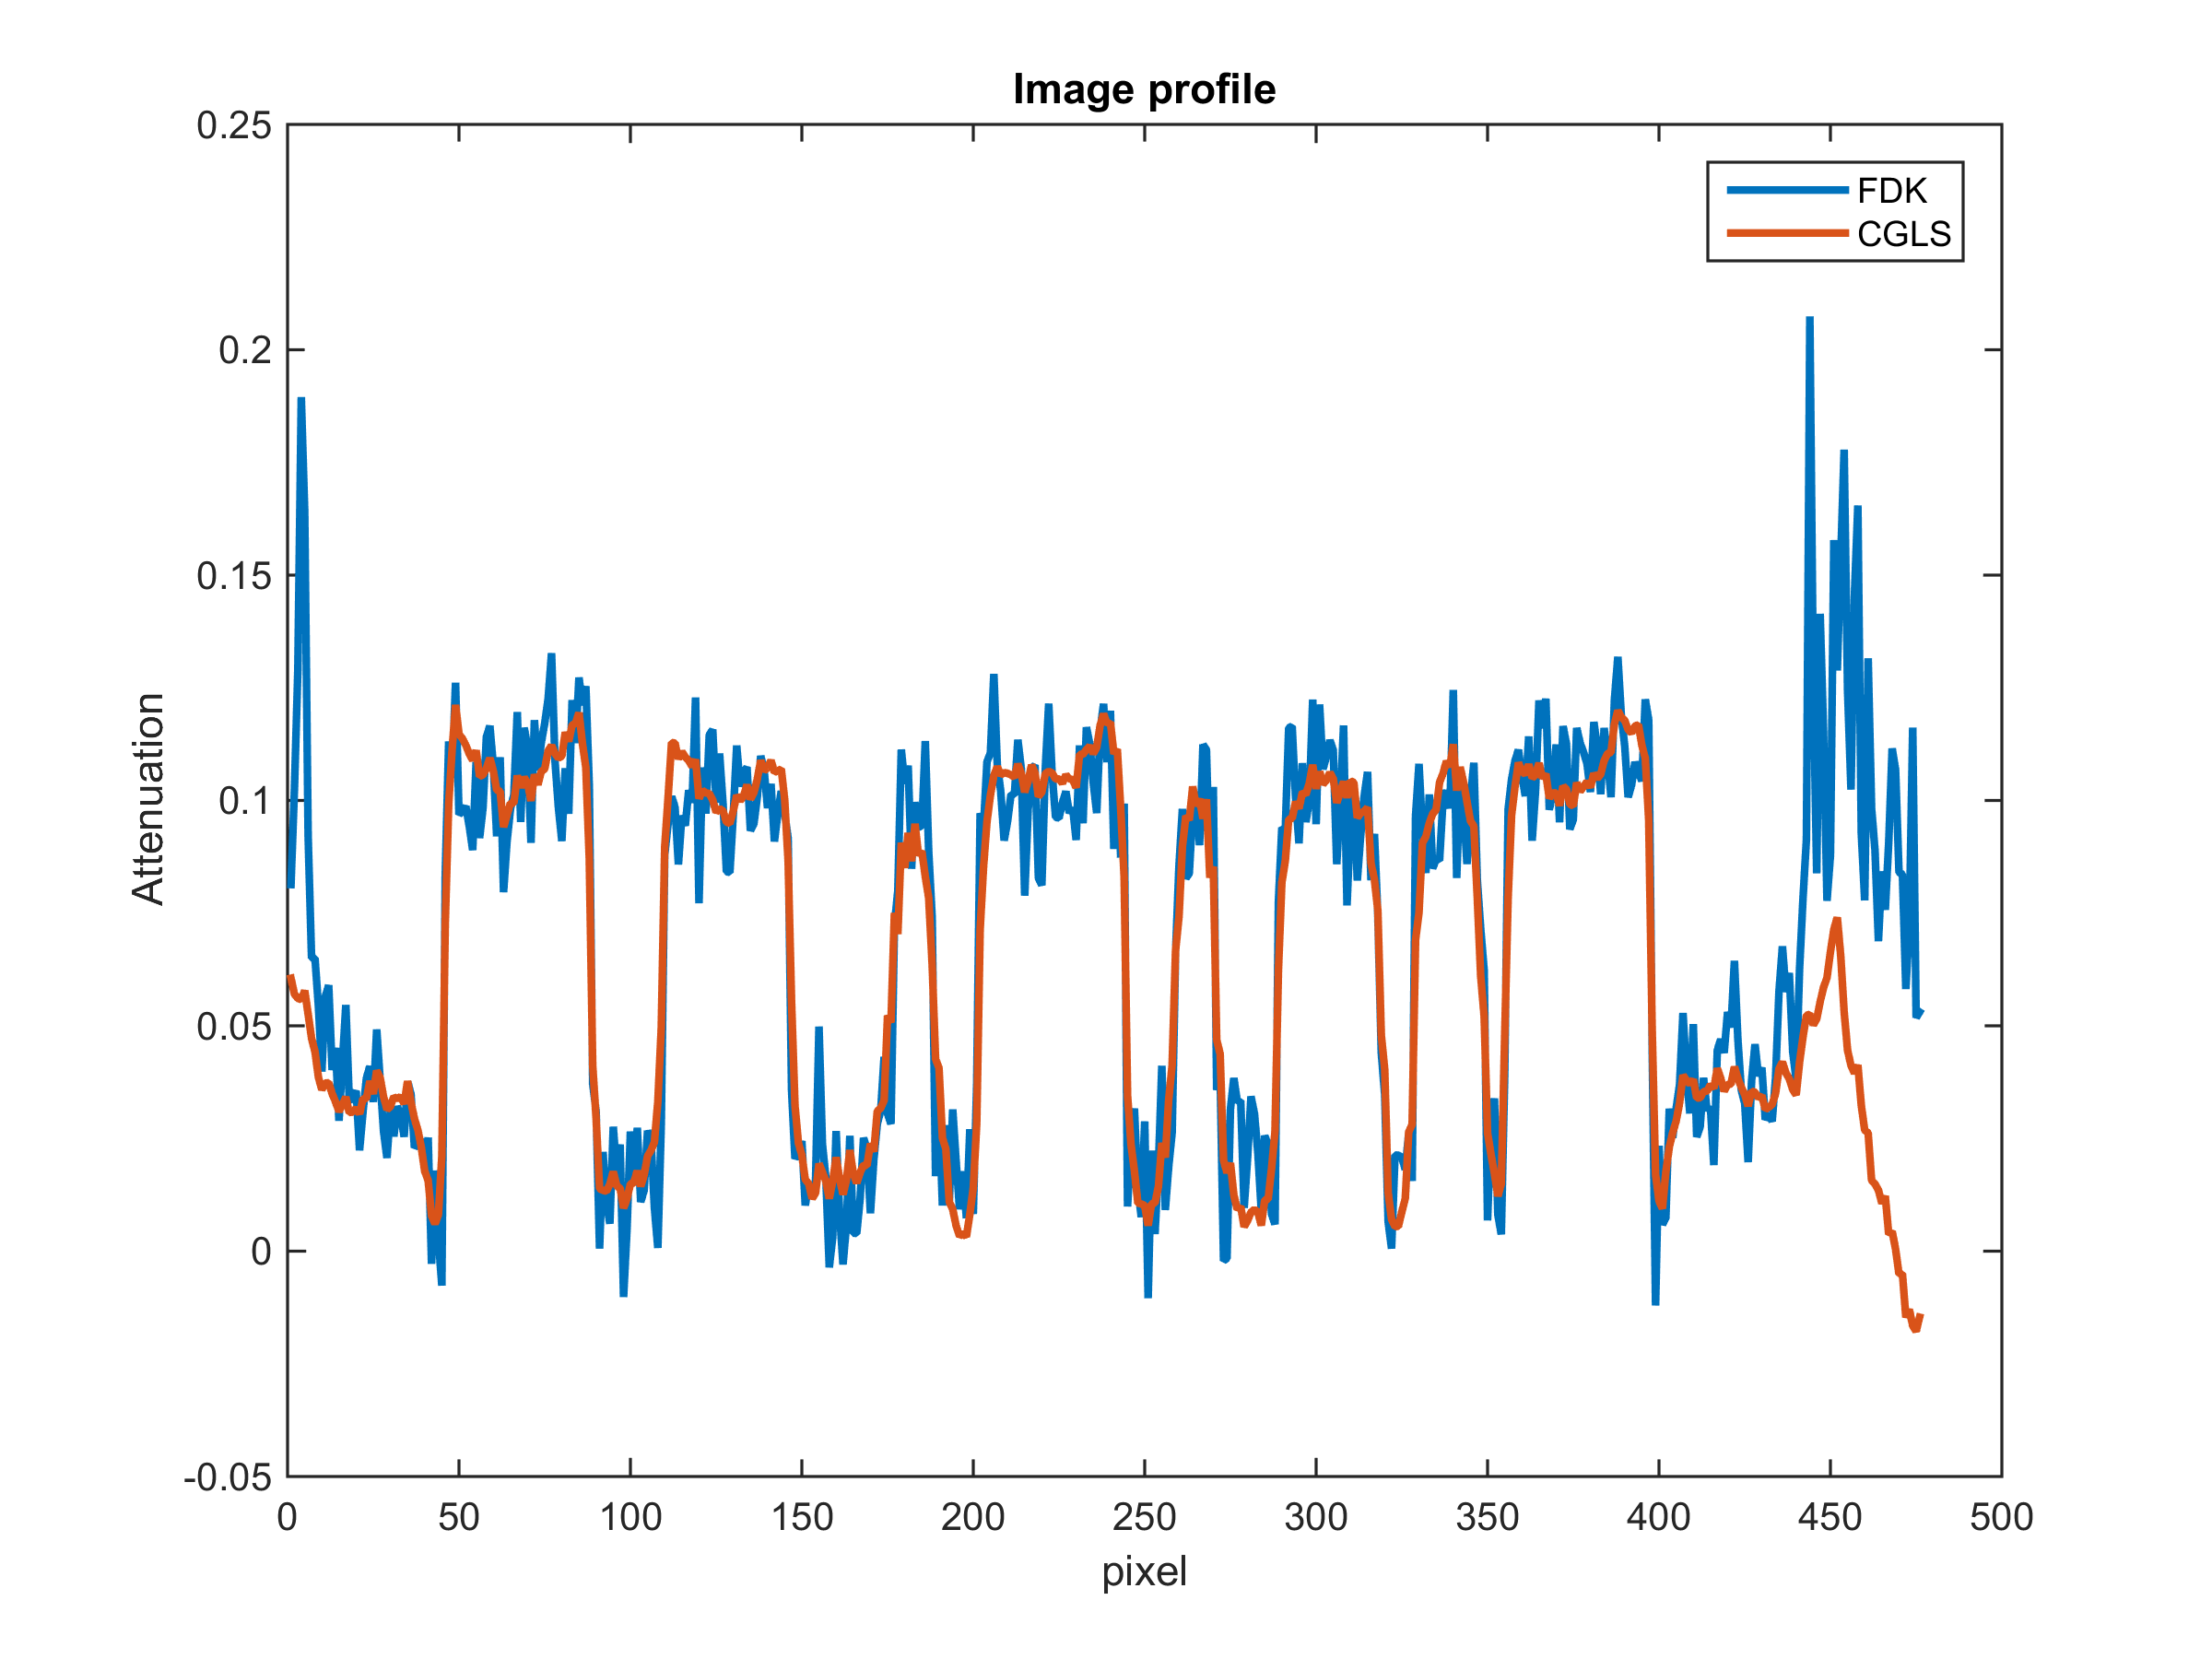
\includegraphics[width=0.65\textwidth]{Applications/spophiaprofile.png} 

\end{center}

\caption[SophiaBeads dataset with FDK and CGLS]{\label{fig:sophiaprofile} Image profile on the SophiaBeads dataset with FDK and CGLS (15 iterations), using 256 projections.} 
\end{figure}


\FloatBarrier
\subsection{Cryo soft X-ray tomography at the Diamond Light Source}

Cryo soft X-ray tomography (Cryo-SXT) is a relatively new technology to image micron size biological samples in full 3D\cite{carzaniga2014cryo}. Generally, cell-imaging is performed with electron microscopy (EM) and all its variants (transmission electron microscopy, scanning electron microscopy, cryo-electron microscopy, electron tomography, etcetera), however these techniques have very limited penetration (less than 1$\mu$m) and thus often require slicing of the samples for volumetric imaging. Cryo-SXT uses the so called water window for X-ray energies around the 500 eV energy range. Unlike at higher energies, where everything is invisible, water becomes transparent but carbon-based tissues are clearly visible in that range. Thus, while with lower resolution than most EM, Cryo-SXT allows full volumetric visualization of the cells without damaging the samples. In order to be able to image with an extremely accurate setup in both sample handling and X-ray parameters, these Cryo-SXT images are captured in synchrotron facilities. The data used in this work is from the B24 beam-line at the Diamond Light Source.

However, Cryo-SXT data has several sources of errors that make its reconstructed images significantly noisy. The typical penetration depth of soft X-rays is around 10 $\mu$m, while the samples are generally an order of magnitude bigger than that in height and width. Thus Cryo-SXT is a limited angle problem, where most of the datasets are sampled over a 120 degree arc. In the extrema of this range, the images in the detector tend to have little or no information for some parts of the sample due to photons not reaching the detector. Additionally, the low intensity and small sample size do mean that the detector data are very noisy, as photons spread out more (at the scale of the pixel dimension) and fewer photons reach the detector. The size of the sample also comes with errors in the mechanical systems of the imaging set up. When working on a scale of microns, any small vibration is visible and considerably perturbs the measured data. Generally these types of errors are removed by pre-processing using alignment techniques, but the algorithms involved are often not fault proof and the data used in reconstruction ends up having some misalignment errors. The datasets in this section has been aligned using IMOD\cite{mastronarde1997dual}. Figure \ref{fig:Cryo-SXT} shows two of the sinograms of the datasets, where the noisy nature of the data can be intermediately appreciated. In the top figure, attenuation artefacts are visible. In the bottom figure, one can see the darkening of the areas at high angles (upper and lower parts of the figure, at 25\% of distance from the left) and areas that have been filled by the alignment algorithm with a single value (mid-left edge and bottom right edge). These last errors do have no influence in filtered backprojection (FBP), as the high-pass filtering of the data sets their values to zero, but they are a source of artefacts in iterative algorithms. Both sinograms show a considerably high amount of random noise.

\begin{figure}
\centering
\begin{tikzpicture}


\node (A) {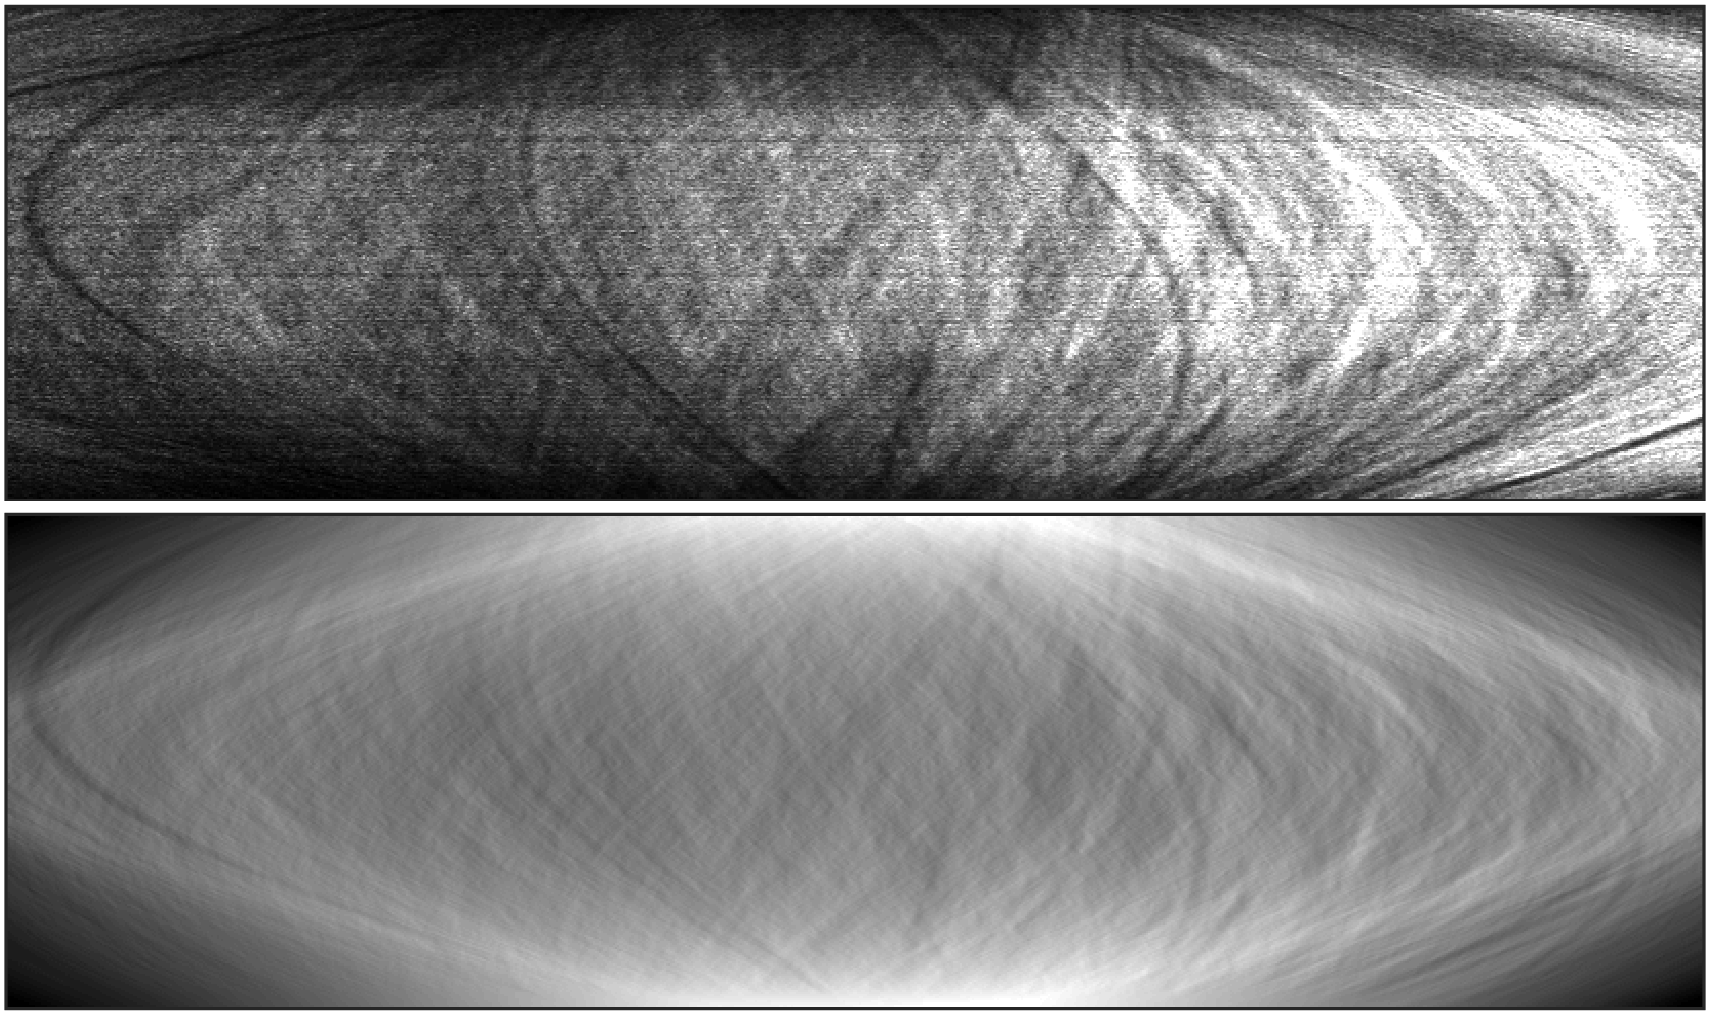
\includegraphics[width=0.9\textwidth]{Applications/sinoqll.png} };
\path (A.south west) -- (A.north west) node[pos=.5, above, rotate=90] {Projection angle};
\path (A.south west) -- (A.south east) node[pos=.5, below] {Horizontal detector pixel};

\end{tikzpicture}

\caption[Sinograms of the data from a Cryo-SXT]{\label{fig:Cryo-SXT} Sinograms of the central slice of two different datasets of the data from a Cryo-SXT. The top figure shows attenuation artefacts over different individual measurements of the data and significant random noise over the whole sinogram. The bottom figure shows strong attenuation at high angles (edges of the image) and artefacts generated by alignment. } 
\end{figure}




A few datasets have been reconstructed from this imaging modality using various algorithms. Objective evaluation of the quality of the reconstructed image with each algorithm is not possible as, due to the noisy nature of the images, classifying some of the visual artefacts as data or noise is hard. Thus this section does not intend to claim that any of the algorithms perform better than FBP, just highlight the differences.

\subsubsection{The ``2017\_0207\_Trypanosoma\_33'' dataset.} This dataset contains a section of an image containing a few Trypanosoma, a unicellular parasitic protozoa that cause different illnesses, such as the sleeping sickness. In the images, the big blob within each of them of similar attenuation level as the rest of the cell is the nucleus, while the smaller circular features are organelles of the cell.

 Several algorithms have been used to test the effect of iterative algorithms.
Initially SIRT and CGLS have been chosen. Both of these algorithms are expected to generate images with very little noise, but perhaps lose the most detailed information, or at least create smoother boundaries than FBP, as they minimize the L2 norm using all data in one go (per iteration). The result of these, compared to FBP can be seen in figure \ref{fig:CGLSSIRT}. SIRT generates a very smooth image without barely any noise, however the details are very smoothed also, specially the boundaries of the objects. However, very few iterations of SIRT have been performed in this dataset. CGLS however seems to separate data from noise better, while also creating some smooth (not as much as SIRT) boundaries. However it is unclear how much of this is caused by misalignments within the data and how much by the algorithms themselves.

As shown earlier in this chapter, OS-SART can improve the convergence speed of SIRT sacrificing some computational time. SART may improve further the convergence, but it becomes a very computational expensive algorithm at this image sizes. Additionally, total variation minimization can be applied to remove the noise that the images have. Figure \ref{fig:OS} shows FBP, OS-SART, and ASD-POCS with 20 total variation iterations and using OS-SART instead of SART as data fidelity update (OS-ASD-POCS).

Note that the images have a darker vertical ``band'', not as obvious in SIRT and CGLS. This is caused by some errors in the projections that with a proper preprocessing step could be removed. OS-SART reconstructs a similar result to FBP, with slightly lower noise levels and extreme values. Fewer iterations of OS-SART would probably generate a less noisy image, however they will also likely show less contrast and features (similar to SIRT before). The total variation version of OS-SART generates a cleaner image, but it has a slight ``watercolour'' texture. The strength of the total variation can be controlled by the number of iterations, increasing them enhances this effect. Figure \ref{fig:OStv} shows 0, 20 and 5 TV iterations. While the tuning of this value can not (yet) be done automatically, once the desired one is found it generally works for all similar images. The actual range of values of the reconstructed voxels is different in each algorithm. This can be explained by the nature of the data, as for example, half of the values are negative, which makes no sense physically. Thus, the visualization range has been adjusted to match histograms of attenuation vale in the figures.


\begin{figure}
\begin{center}

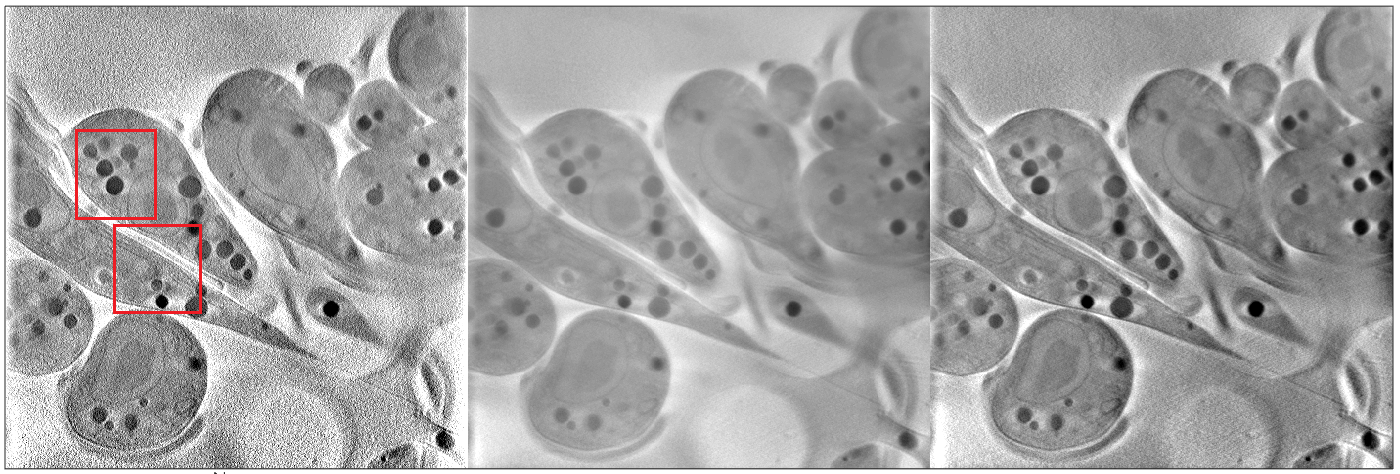
\includegraphics[width=\textwidth]{Applications/FBP_SIRT_CGLSm.png} 
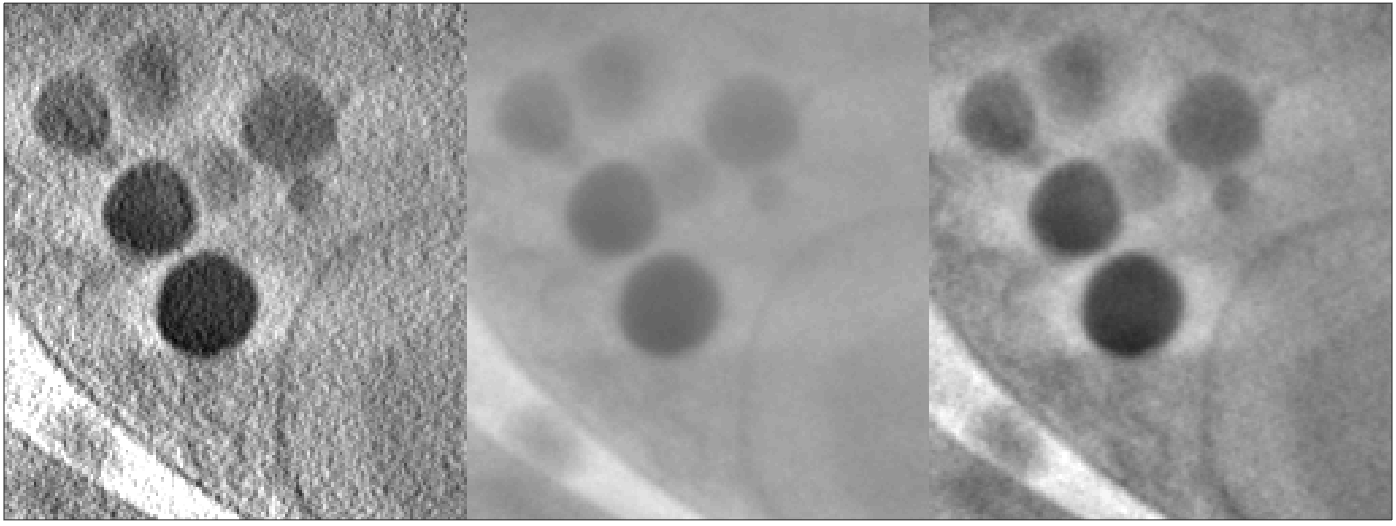
\includegraphics[width=\textwidth]{Applications/FBP_SIRT_CGLSz1.png} 
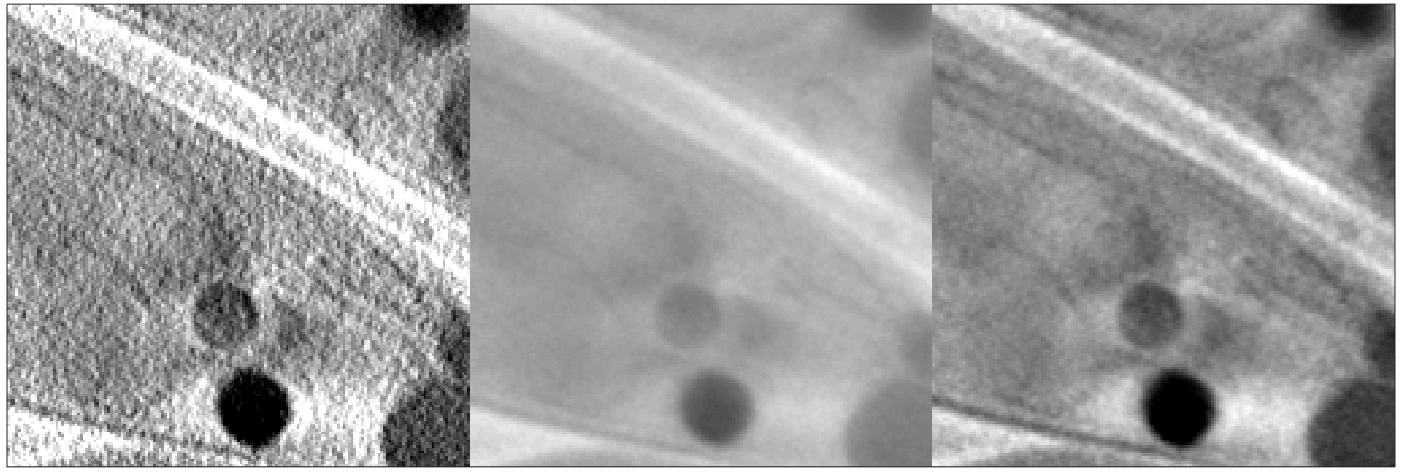
\includegraphics[width=\textwidth]{Applications/FBP_SIRT_CGLSz2.png} 

\end{center}

\caption[Cell image recosntructed with different algorithms 1-1]{\label{fig:CGLSSIRT} Columns: FBP, SIRT (20 iterations) and CGLS (7 iterations). The red squares in the first row show the location of the zoomed-in areas from the second and third row.} 
\end{figure}


\begin{figure}
\begin{center}

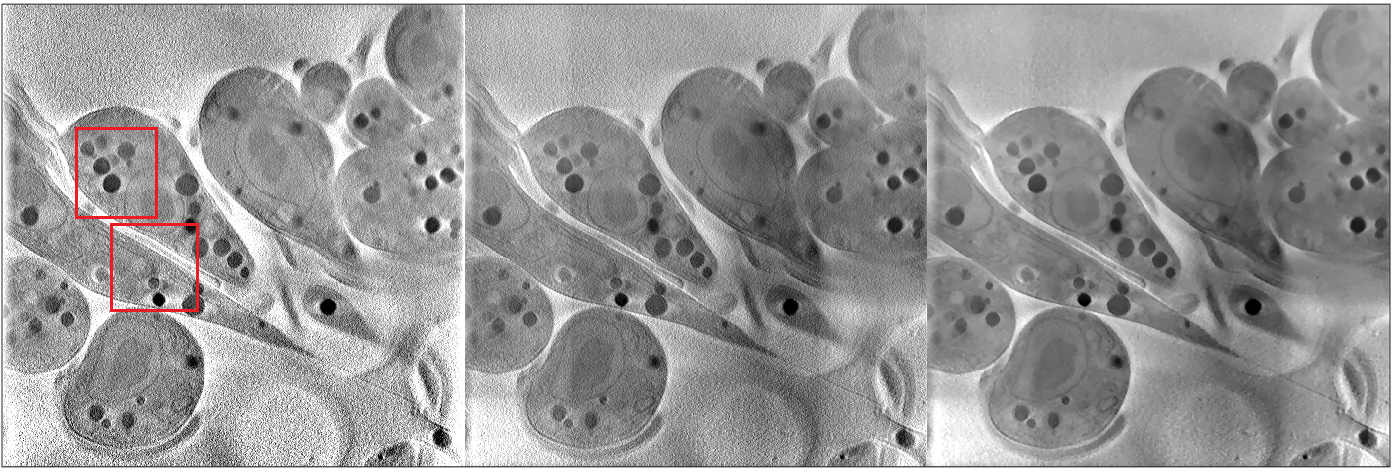
\includegraphics[width=\textwidth]{Applications/FBP_OSSART_TV.png} 
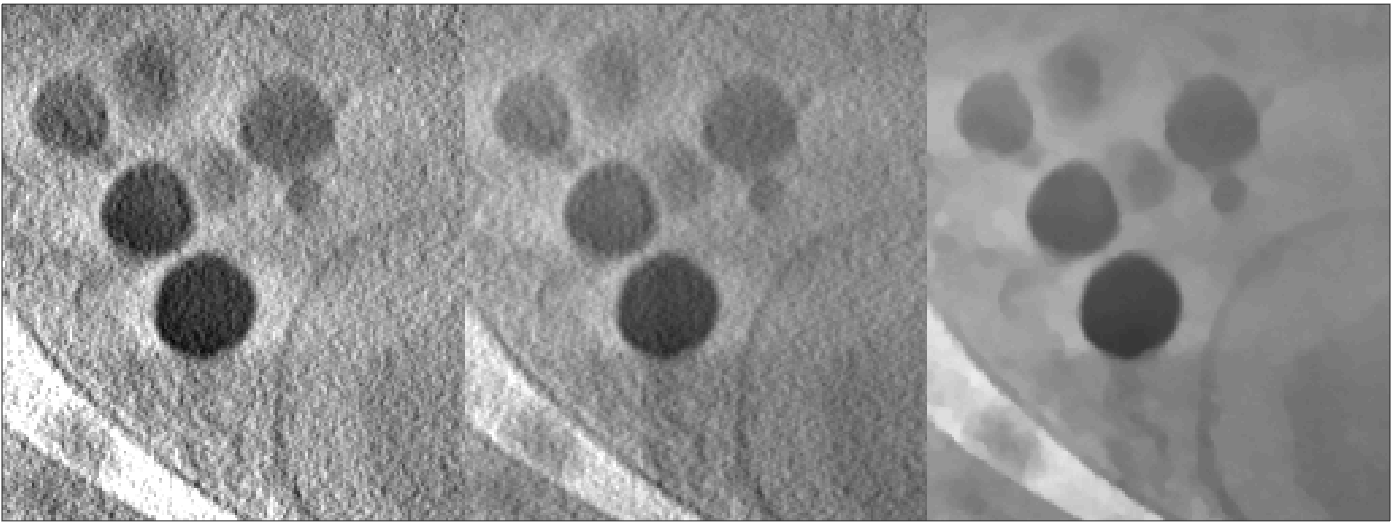
\includegraphics[width=\textwidth]{Applications/FBP_OSSART_TVz1.png} 
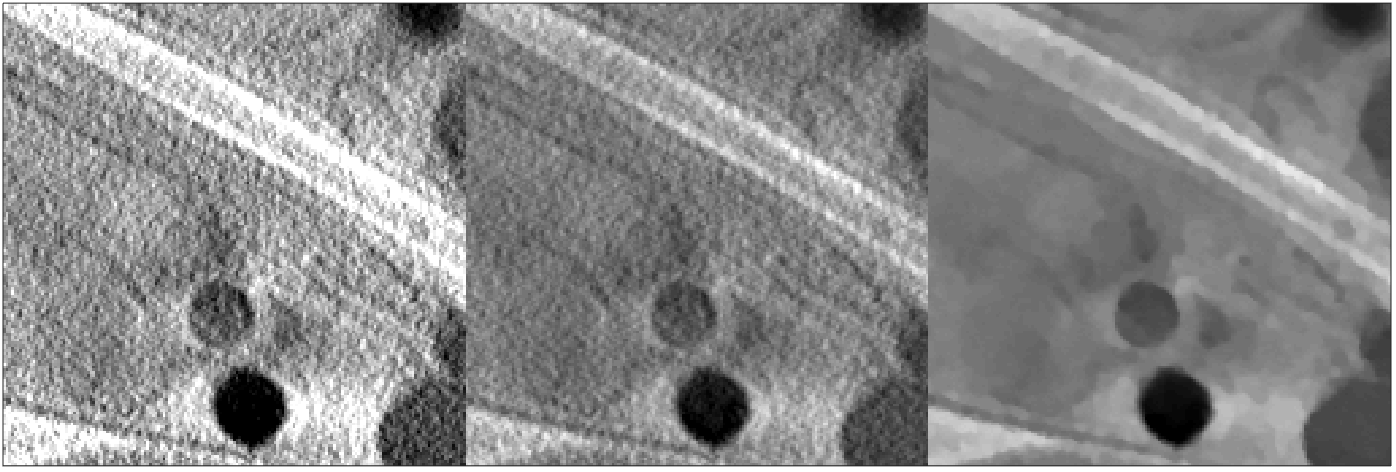
\includegraphics[width=\textwidth]{Applications/FBP_OSSART_TVz2.png} 

\end{center}

\caption[Cell image recosntructed with different algorithms 1-2]{\label{fig:OS}Columns: FBP, OS-SART (20 iterations) and OS-ASD-POCS (20 iterations, 20 TV iterations each). The red squares in the first row show the location of the zoomed-in areas from the second and third row.} 
\end{figure}


\begin{figure}
\begin{center}

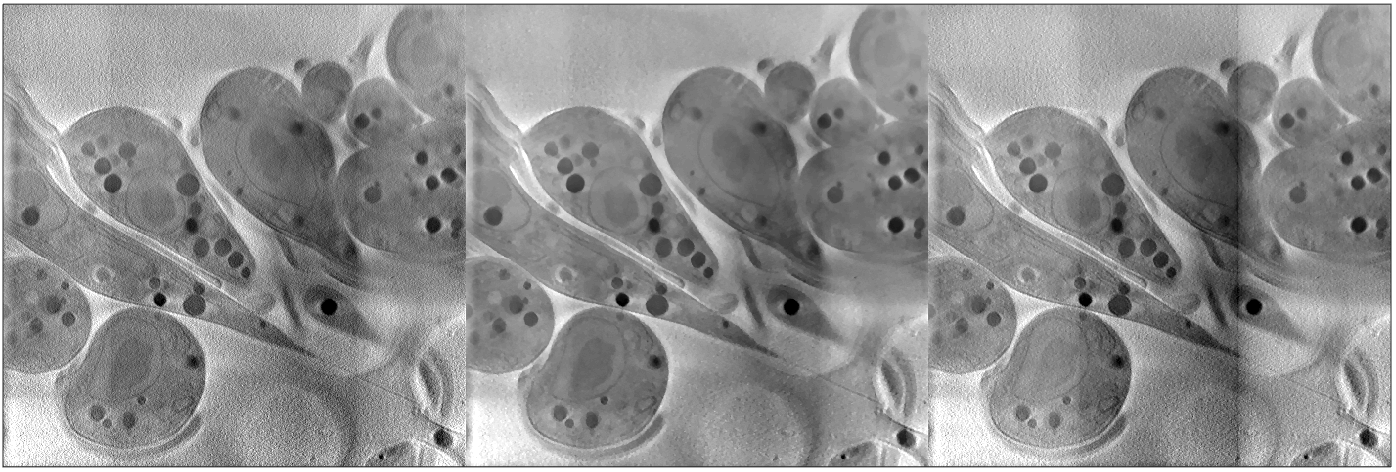
\includegraphics[width=\textwidth]{Applications/OSSART_0_20_5_TViters.png} 
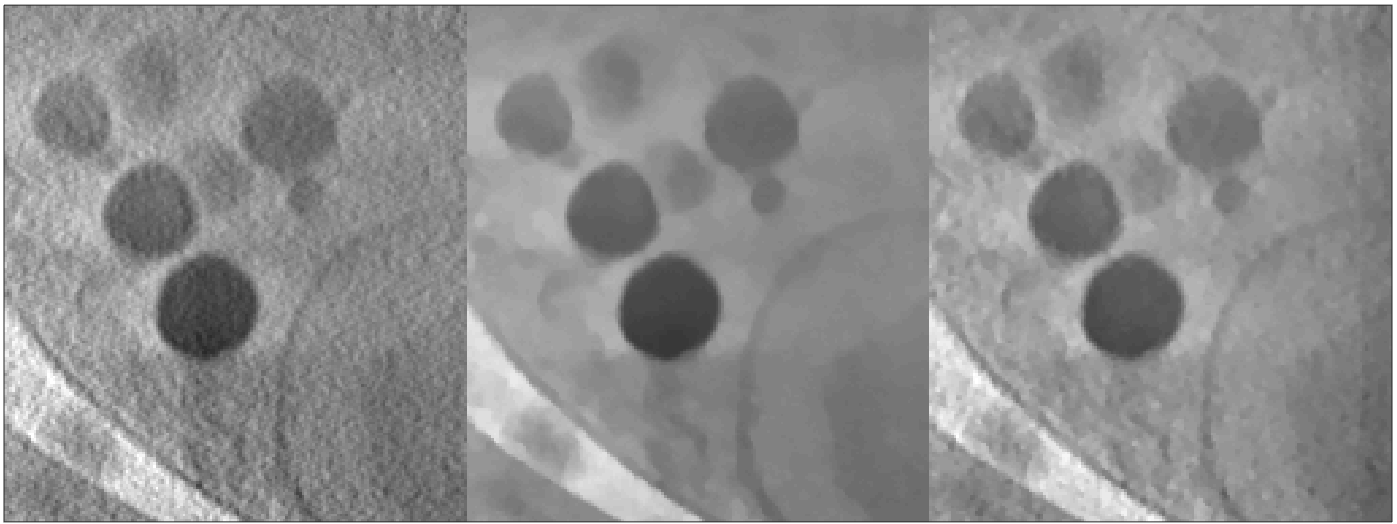
\includegraphics[width=\textwidth]{Applications/OSSART_0_20_5_TVitersz1.png} 
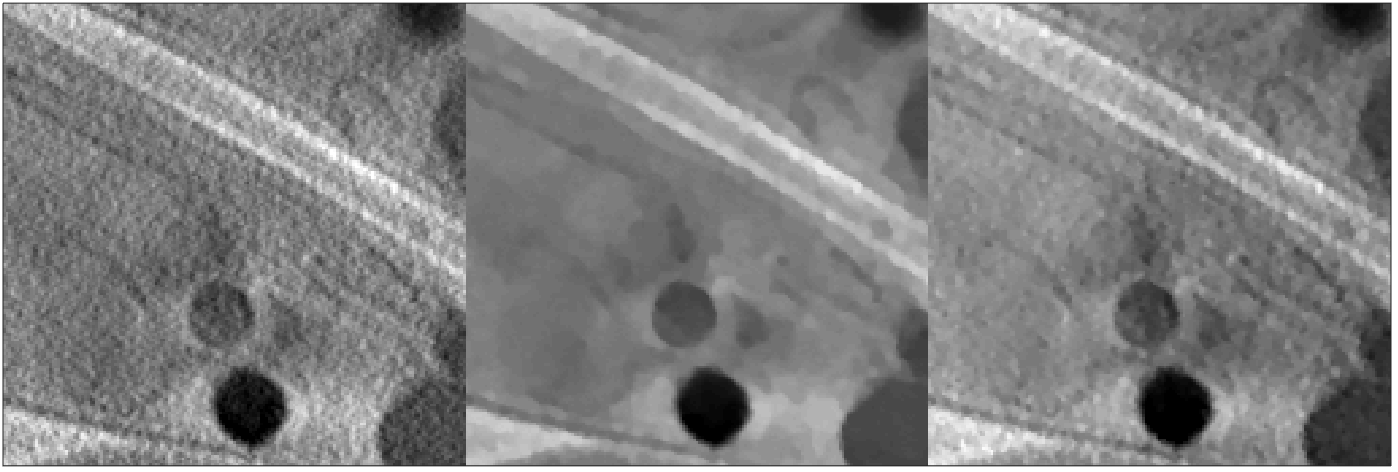
\includegraphics[width=\textwidth]{Applications/OSSART_0_20_5_TVitersz2.png} 

\end{center}

\caption[Cell image recosntructed with different algorithms 1-3]{\label{fig:OStv}Columns: OS-SART (20 iterations, 0 TV iterations), OS-ASD-POCS (20 iterations, 20 TV iterations each), OS-ASD-POCS (20 iterations, 5 TV iterations each). The red squares in the first row show the location of the zoomed-in areas from the second and third row.} 
\end{figure}

\FloatBarrier

\subsubsection{The ``3\_20160218\_tomo\_65t55\_p5\_area\_2MB1\_Export'' dataset.} This dataset contains, as described by Luengo \textit{et al}\cite{LUENGO201743} the zoomed area of a ``neuronal-like mammalian cell line (PC-12\cite{apostol2003cell}).'' The article has more information on the preparation of the samples.

 The big smooth area in the top left side is the nucleus of the cell, while the rest are organelles on the cytoplasm of the cell.  In figure \ref{fig:Diamond2} the reconstructed image can be seen, on where the columns show FBP, OS-SART, CGLS and OS-ASD-POCS algorithms, and the rows different zoomed areas of the image. Due to hinger noise in the projections, the iterative algorithms to have a strong influence in the removal of the noise in this dataset. This is clearly apparent in the second row of the figure \ref{fig:Diamond2}, on where the three iterative algorithms, specially the TV based one, remove significantly the noise of the organelles both in the left and right side of the image. 

\subsubsection{The ``Grid1\_Area2\_Cell2\_tomo3-All\_60t60\_p5d\_6s\_mb1\_Export'' dataset}
This images also show a PC-12 cell, with part nucleus and part organelles, as in the previous dataset. The same algorithms have been used, and the results can be seen in figure \ref{fig:Diamond3}. Tho further try to evaluate the quality of the reconstruction, the Super-Region Volume Segmentation (SuRVoS)\cite{LUENGO201743} workbench is used on this dataset. SuRVoS is an image segmentation workbench designed for X-ray images such as this ones, where classic segmentation techniques do not work due to the noisy nature of the data. SuRVoS takes few manually labelled areas in the image and attempts to segment and label the entire image based on that, using machine learning techniques. Figure \ref{fig:survos} shows automatic segmentation of the cell for FBP and OS-ASD-POCS. OS-ASD-POCS results in a different segmentation for the boundary between the nucleus and the rest of the cell (purple-green boundary) by leaving the wall in the opposite side than FBP, and has some error in the bottom zoomed area. However, organelles (pink) are segmented with a better shape, and less mislabelling happens as last 2 zoomed areas have both mislabelled areas in FBP that are not present in OS-ASD-POCS.



\begin{figure}
\begin{center}

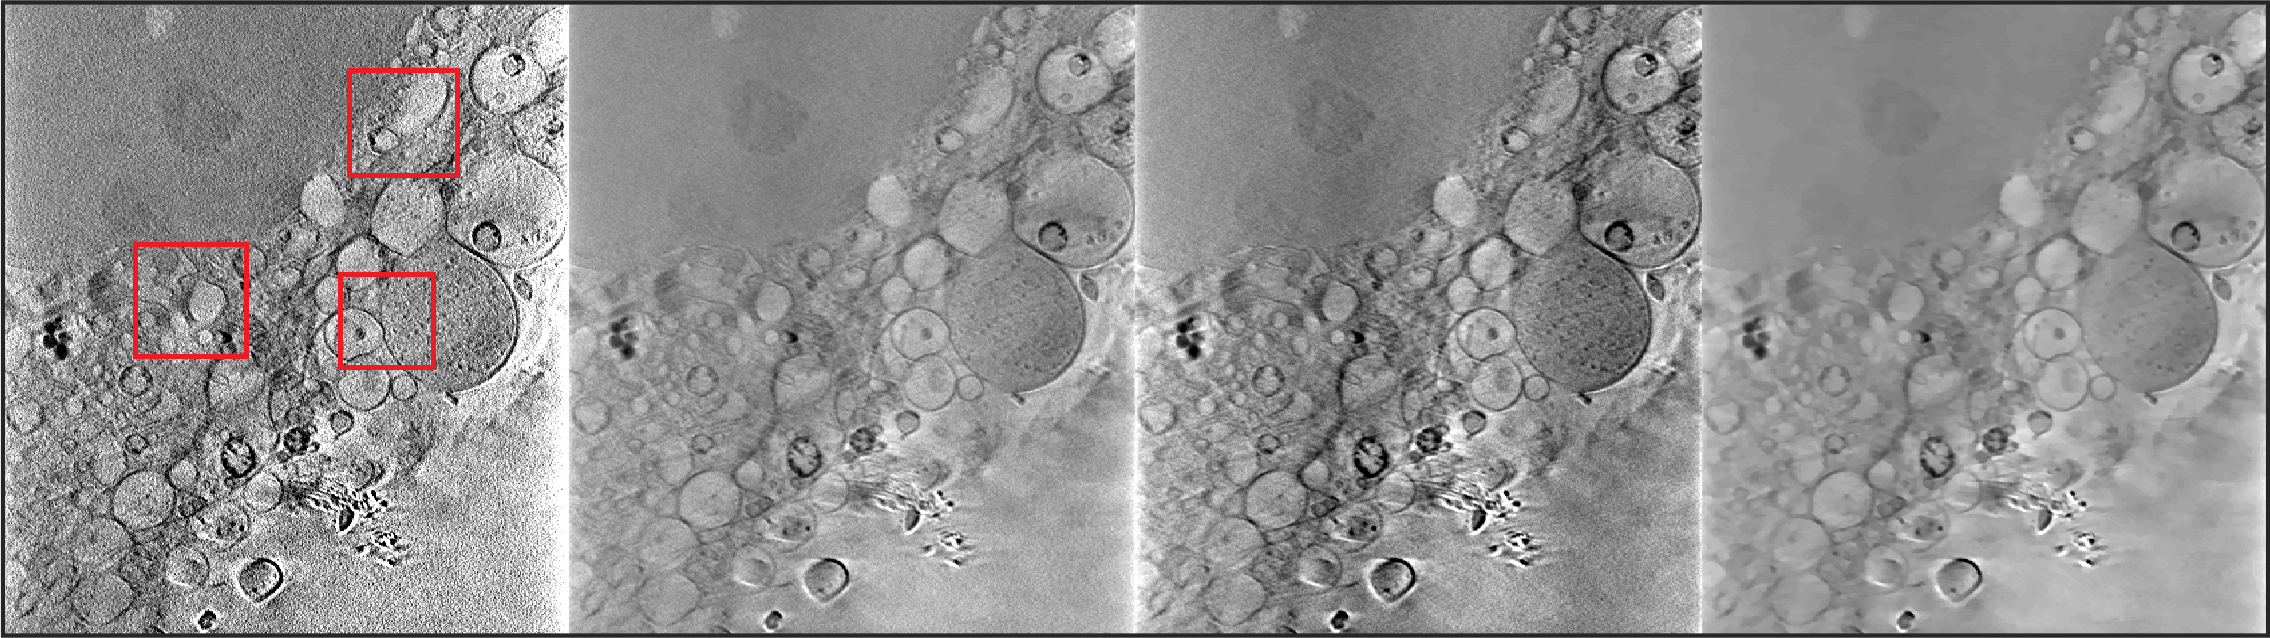
\includegraphics[width=\textwidth]{Applications/Diamond1_full_marked.png} 
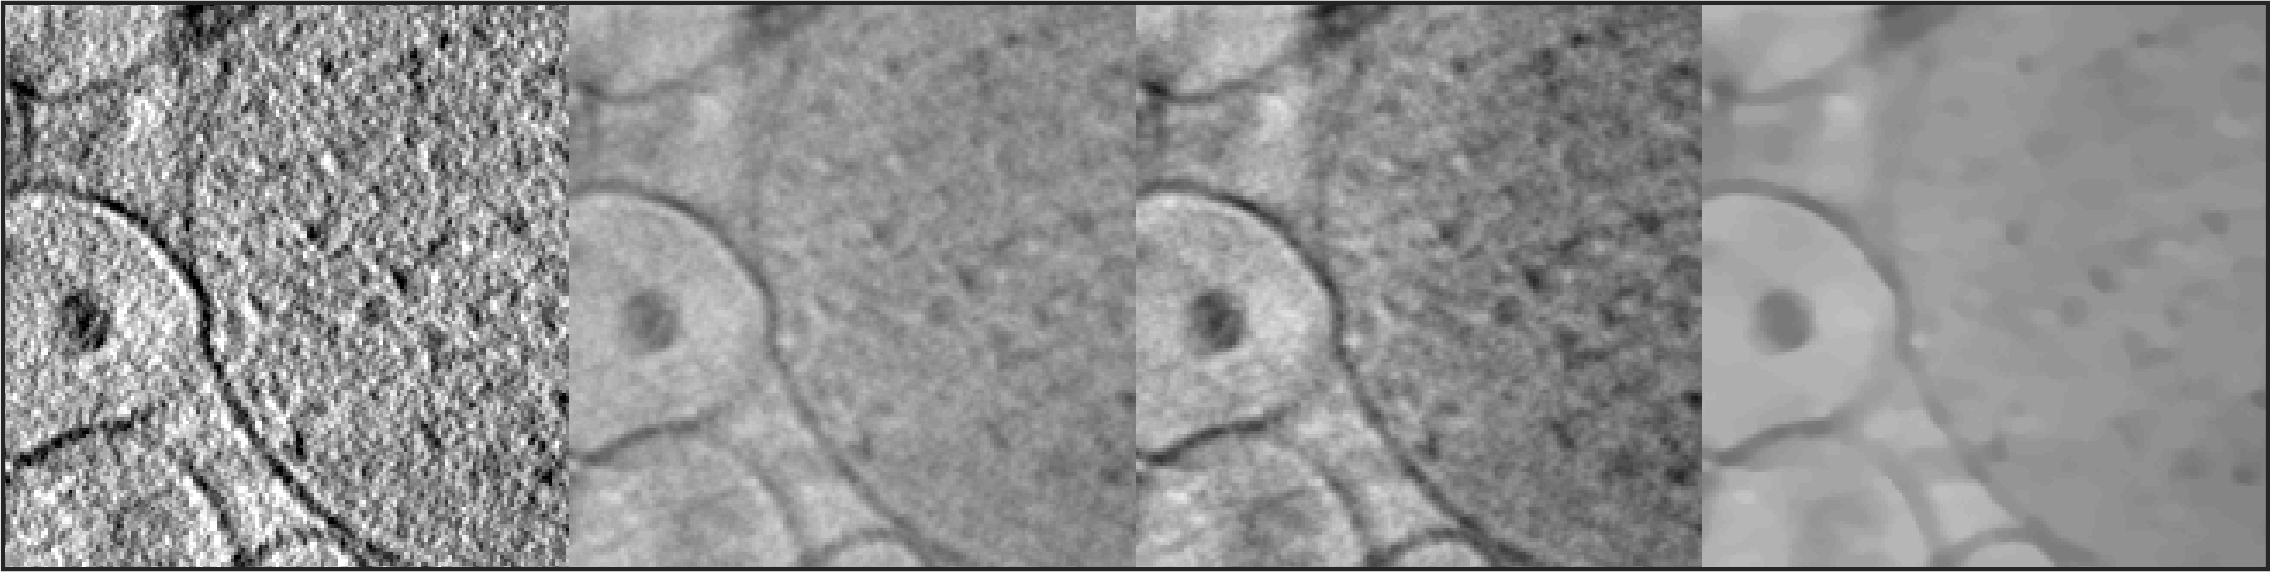
\includegraphics[width=\textwidth]{Applications/Diamond1zoom1.png} 
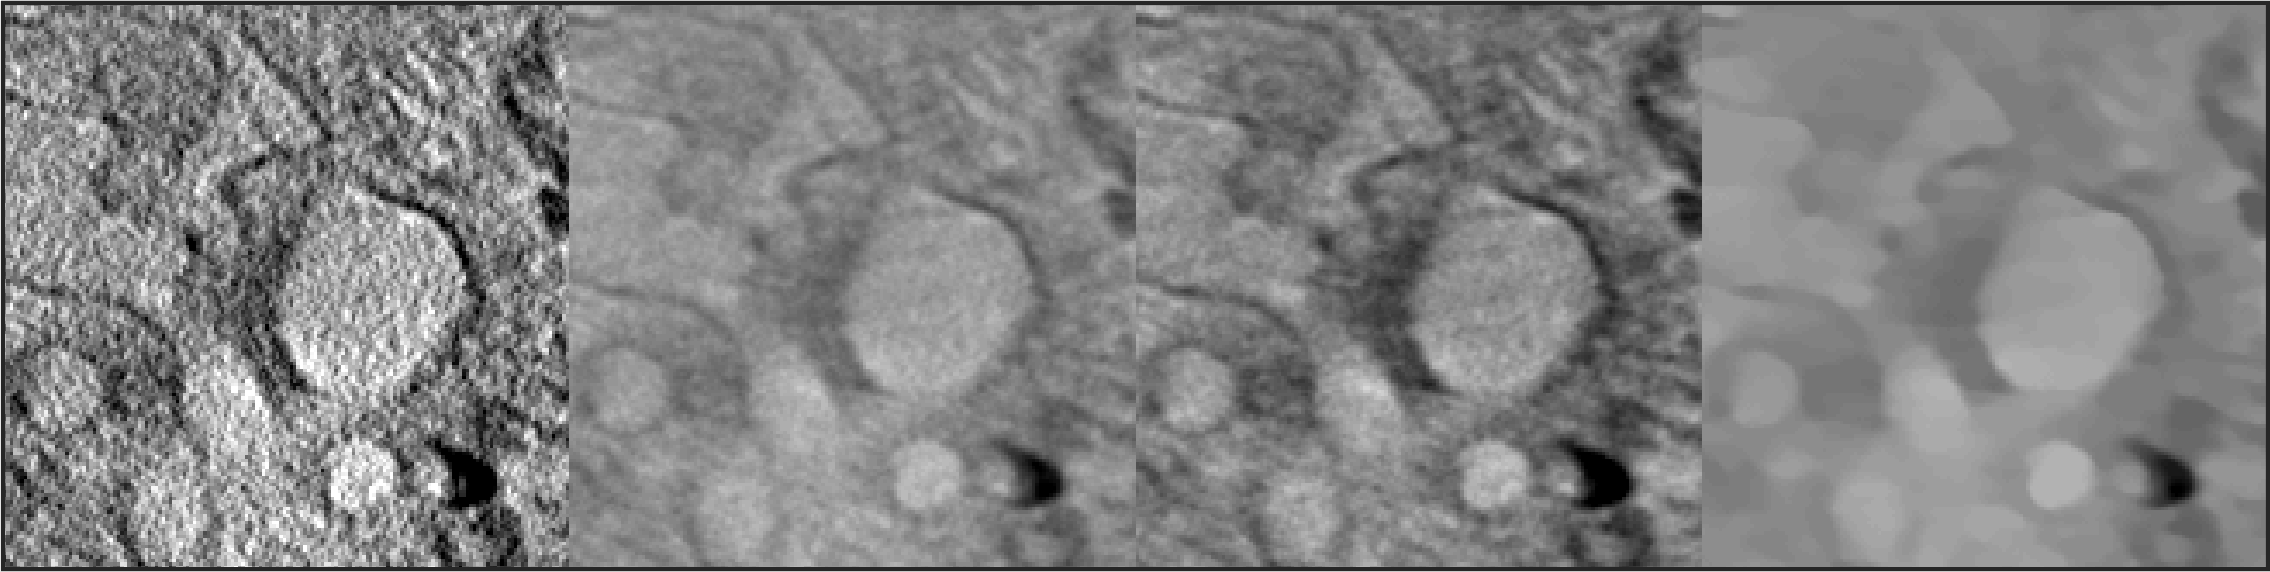
\includegraphics[width=\textwidth]{Applications/Diamond1zoom2.png} 
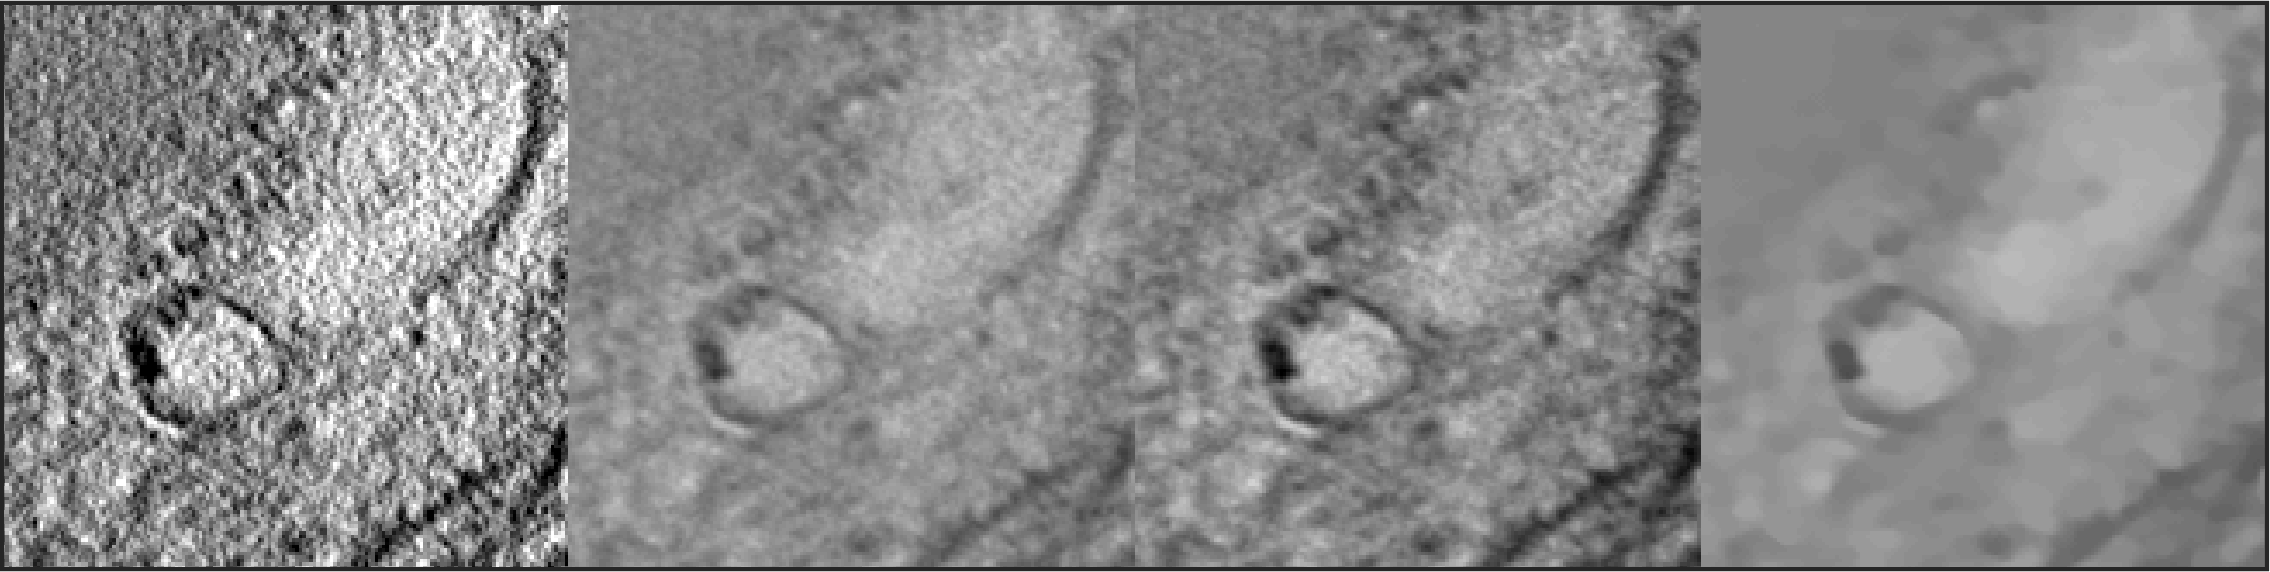
\includegraphics[width=\textwidth]{Applications/Diamond1zoom3.png} 

\end{center}

\caption[Cell image recosntructed with different algorithms 2]{\label{fig:Diamond2} Columns: FBP, OS-SART (30 iterations), CGLS (7 iterations) and OS-ASD-POCS (30 iterations, 10 TV iterations each). The zoomed areas are highlighted in the FBP image.  The red squares in the first row show the location of the zoomed-in areas from the second third and fourth row.} 
\end{figure}
\begin{figure}
\begin{center}

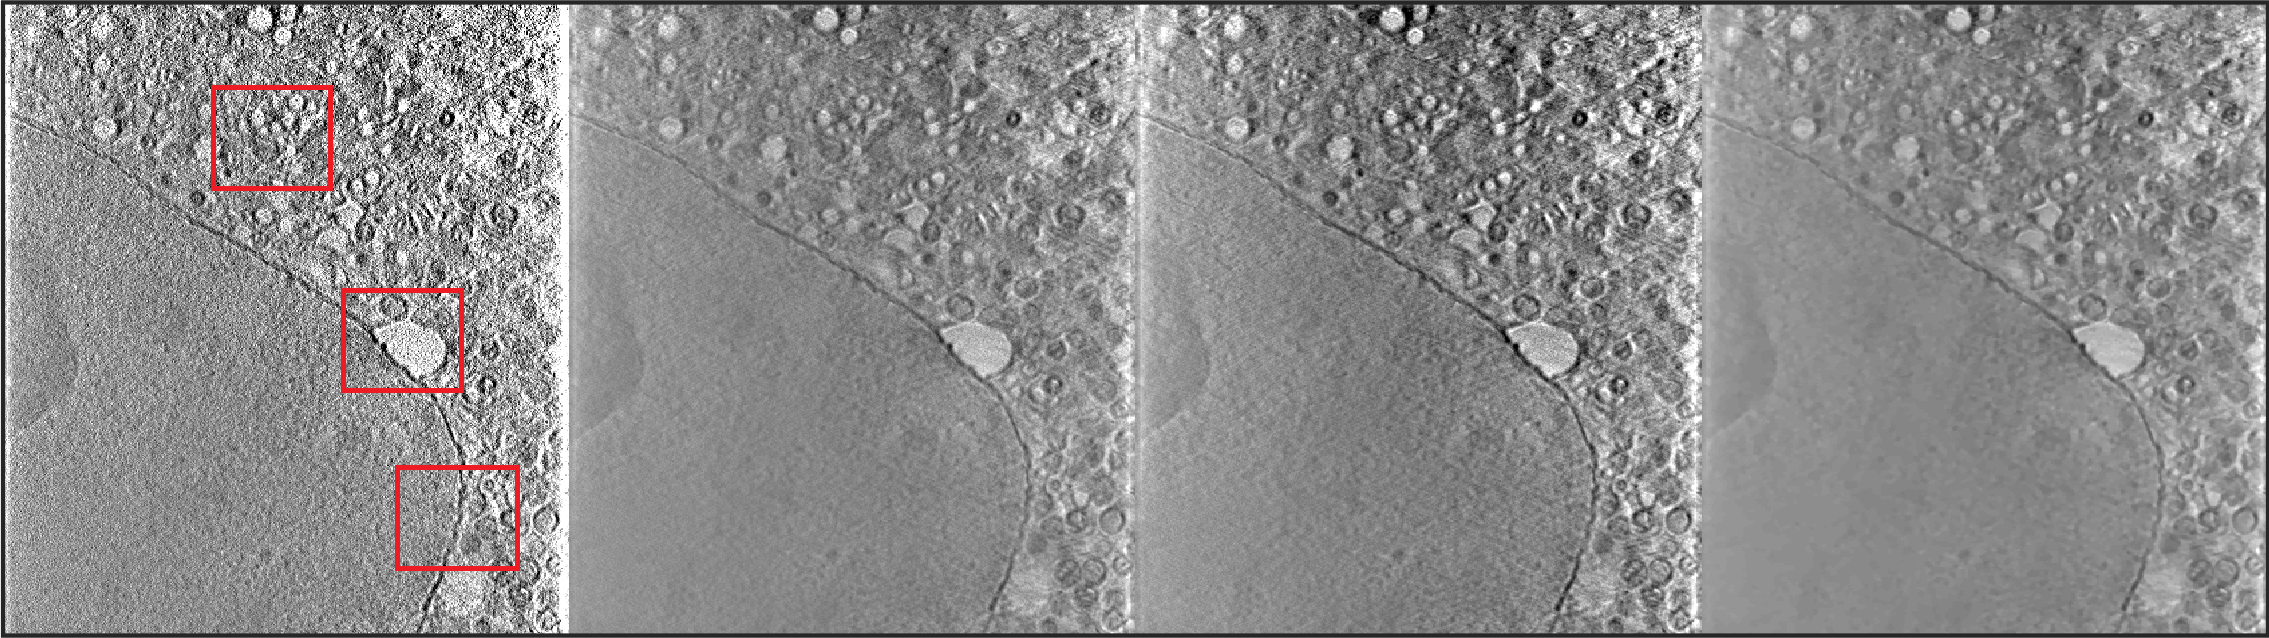
\includegraphics[width=\textwidth]{Applications/Diamond5.png} 
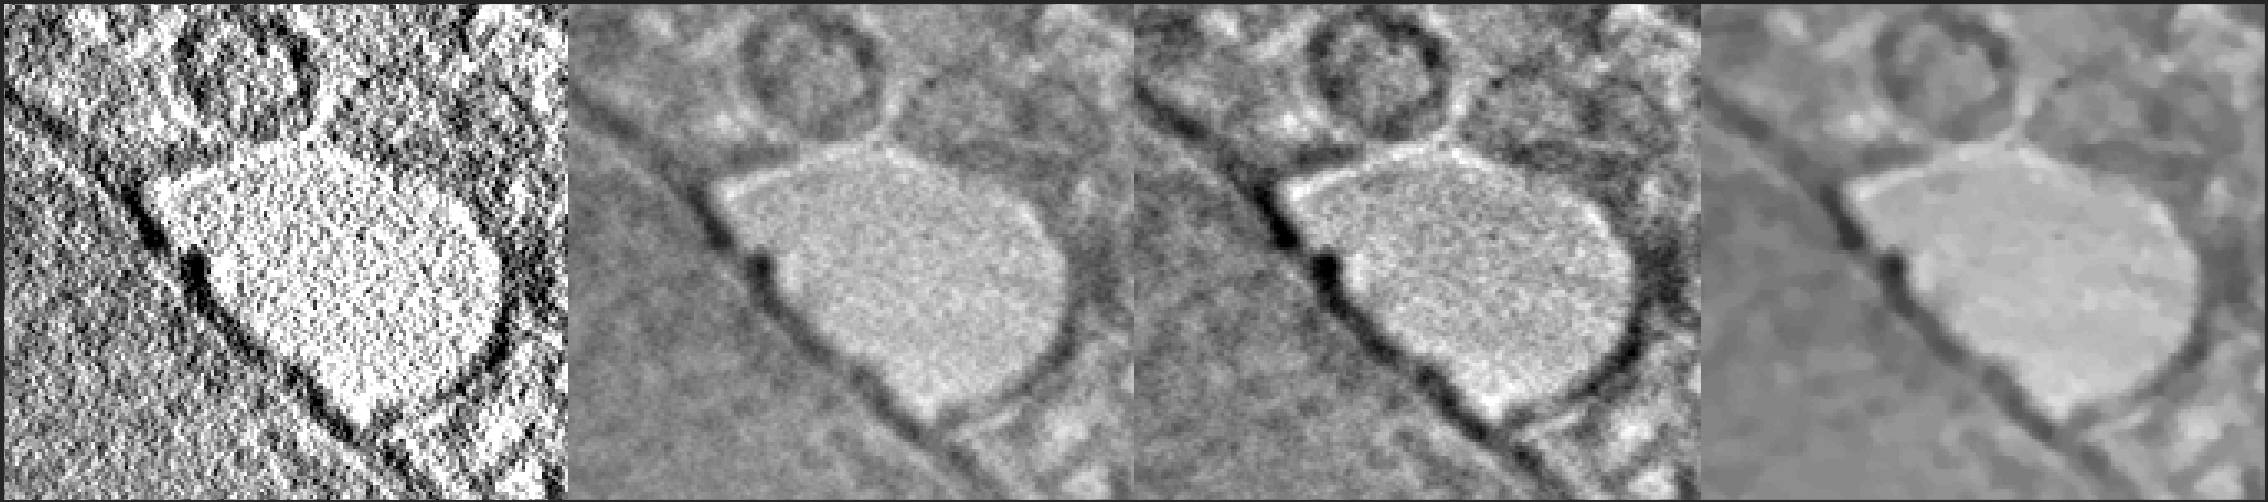
\includegraphics[width=\textwidth]{Applications/Diamond5zoom1.png} 
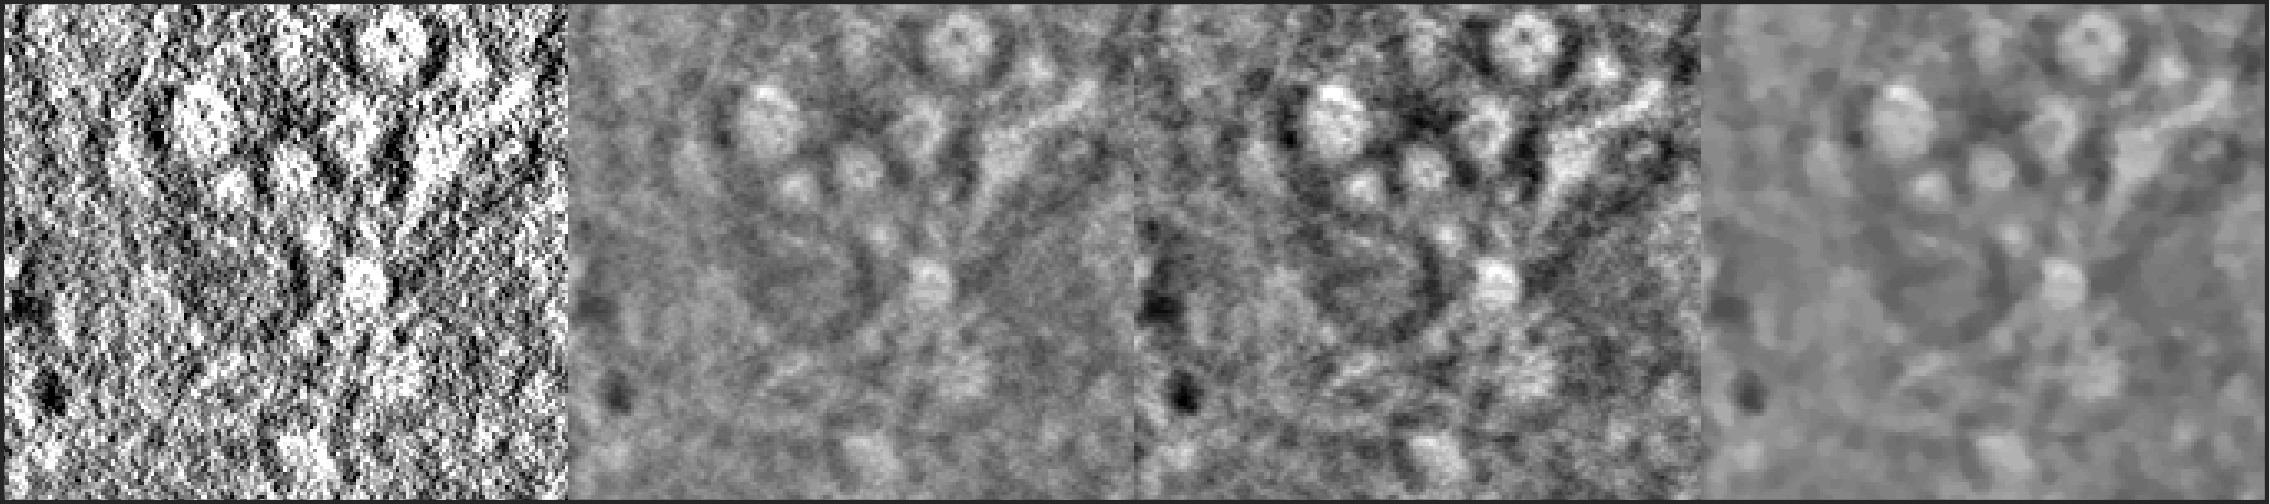
\includegraphics[width=\textwidth]{Applications/Diamond5zoom2.png} 
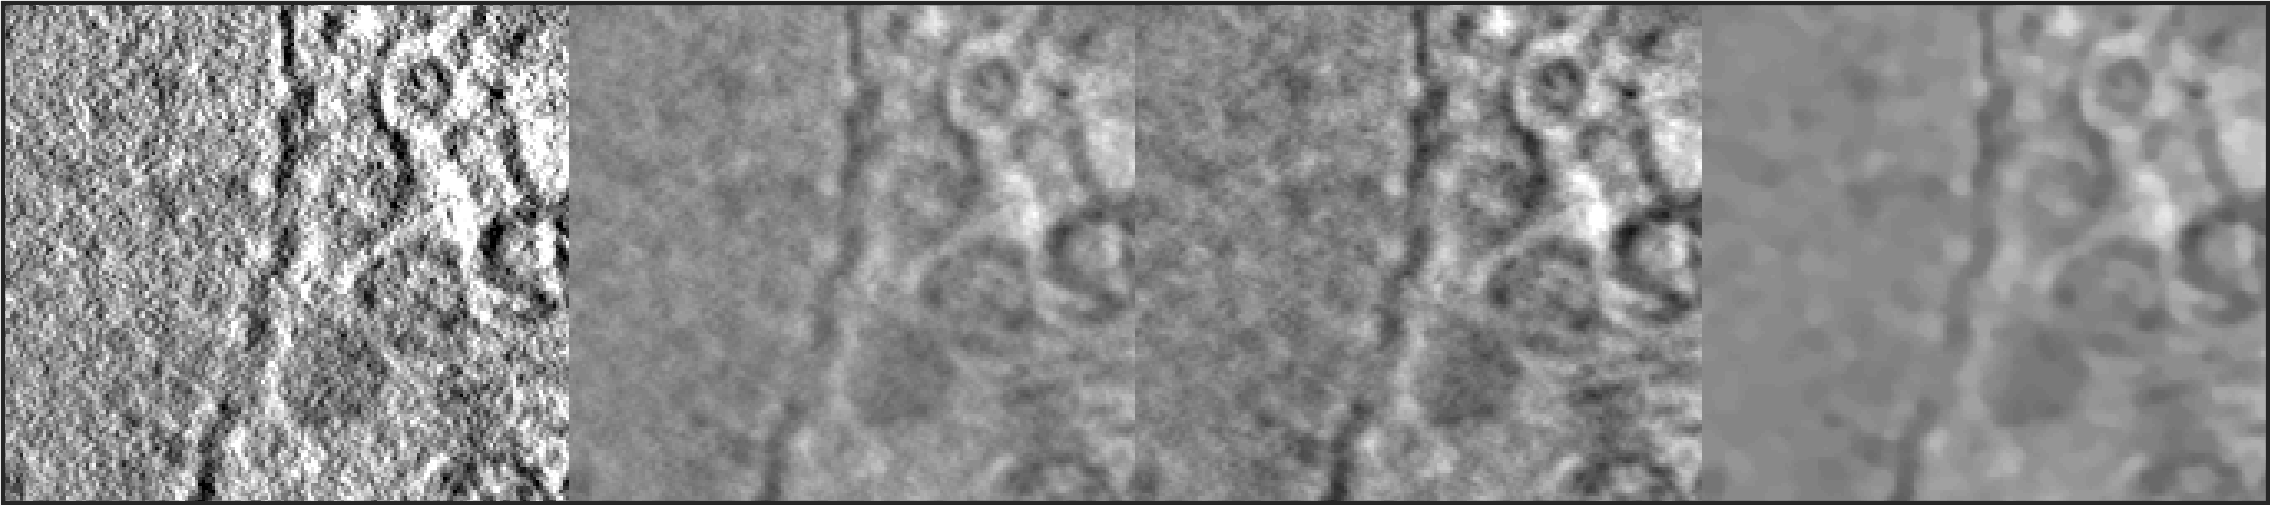
\includegraphics[width=\textwidth]{Applications/Diamond5zoom3.png} 

\end{center}

\caption[Cell image recosntructed with different algorithms 3]{\label{fig:Diamond3} Columns: FBP, OS-SART (30 iterations), CGLS (7 iterations) and OS-ASD-POCS (30 iterations, 10 TV iterations each). The zoomed areas are highlighted in the FBP image. The red squares in the first row show the location of the zoomed-in areas from the second third and fourth row.} 
\end{figure}


\begin{figure}
\begin{center}

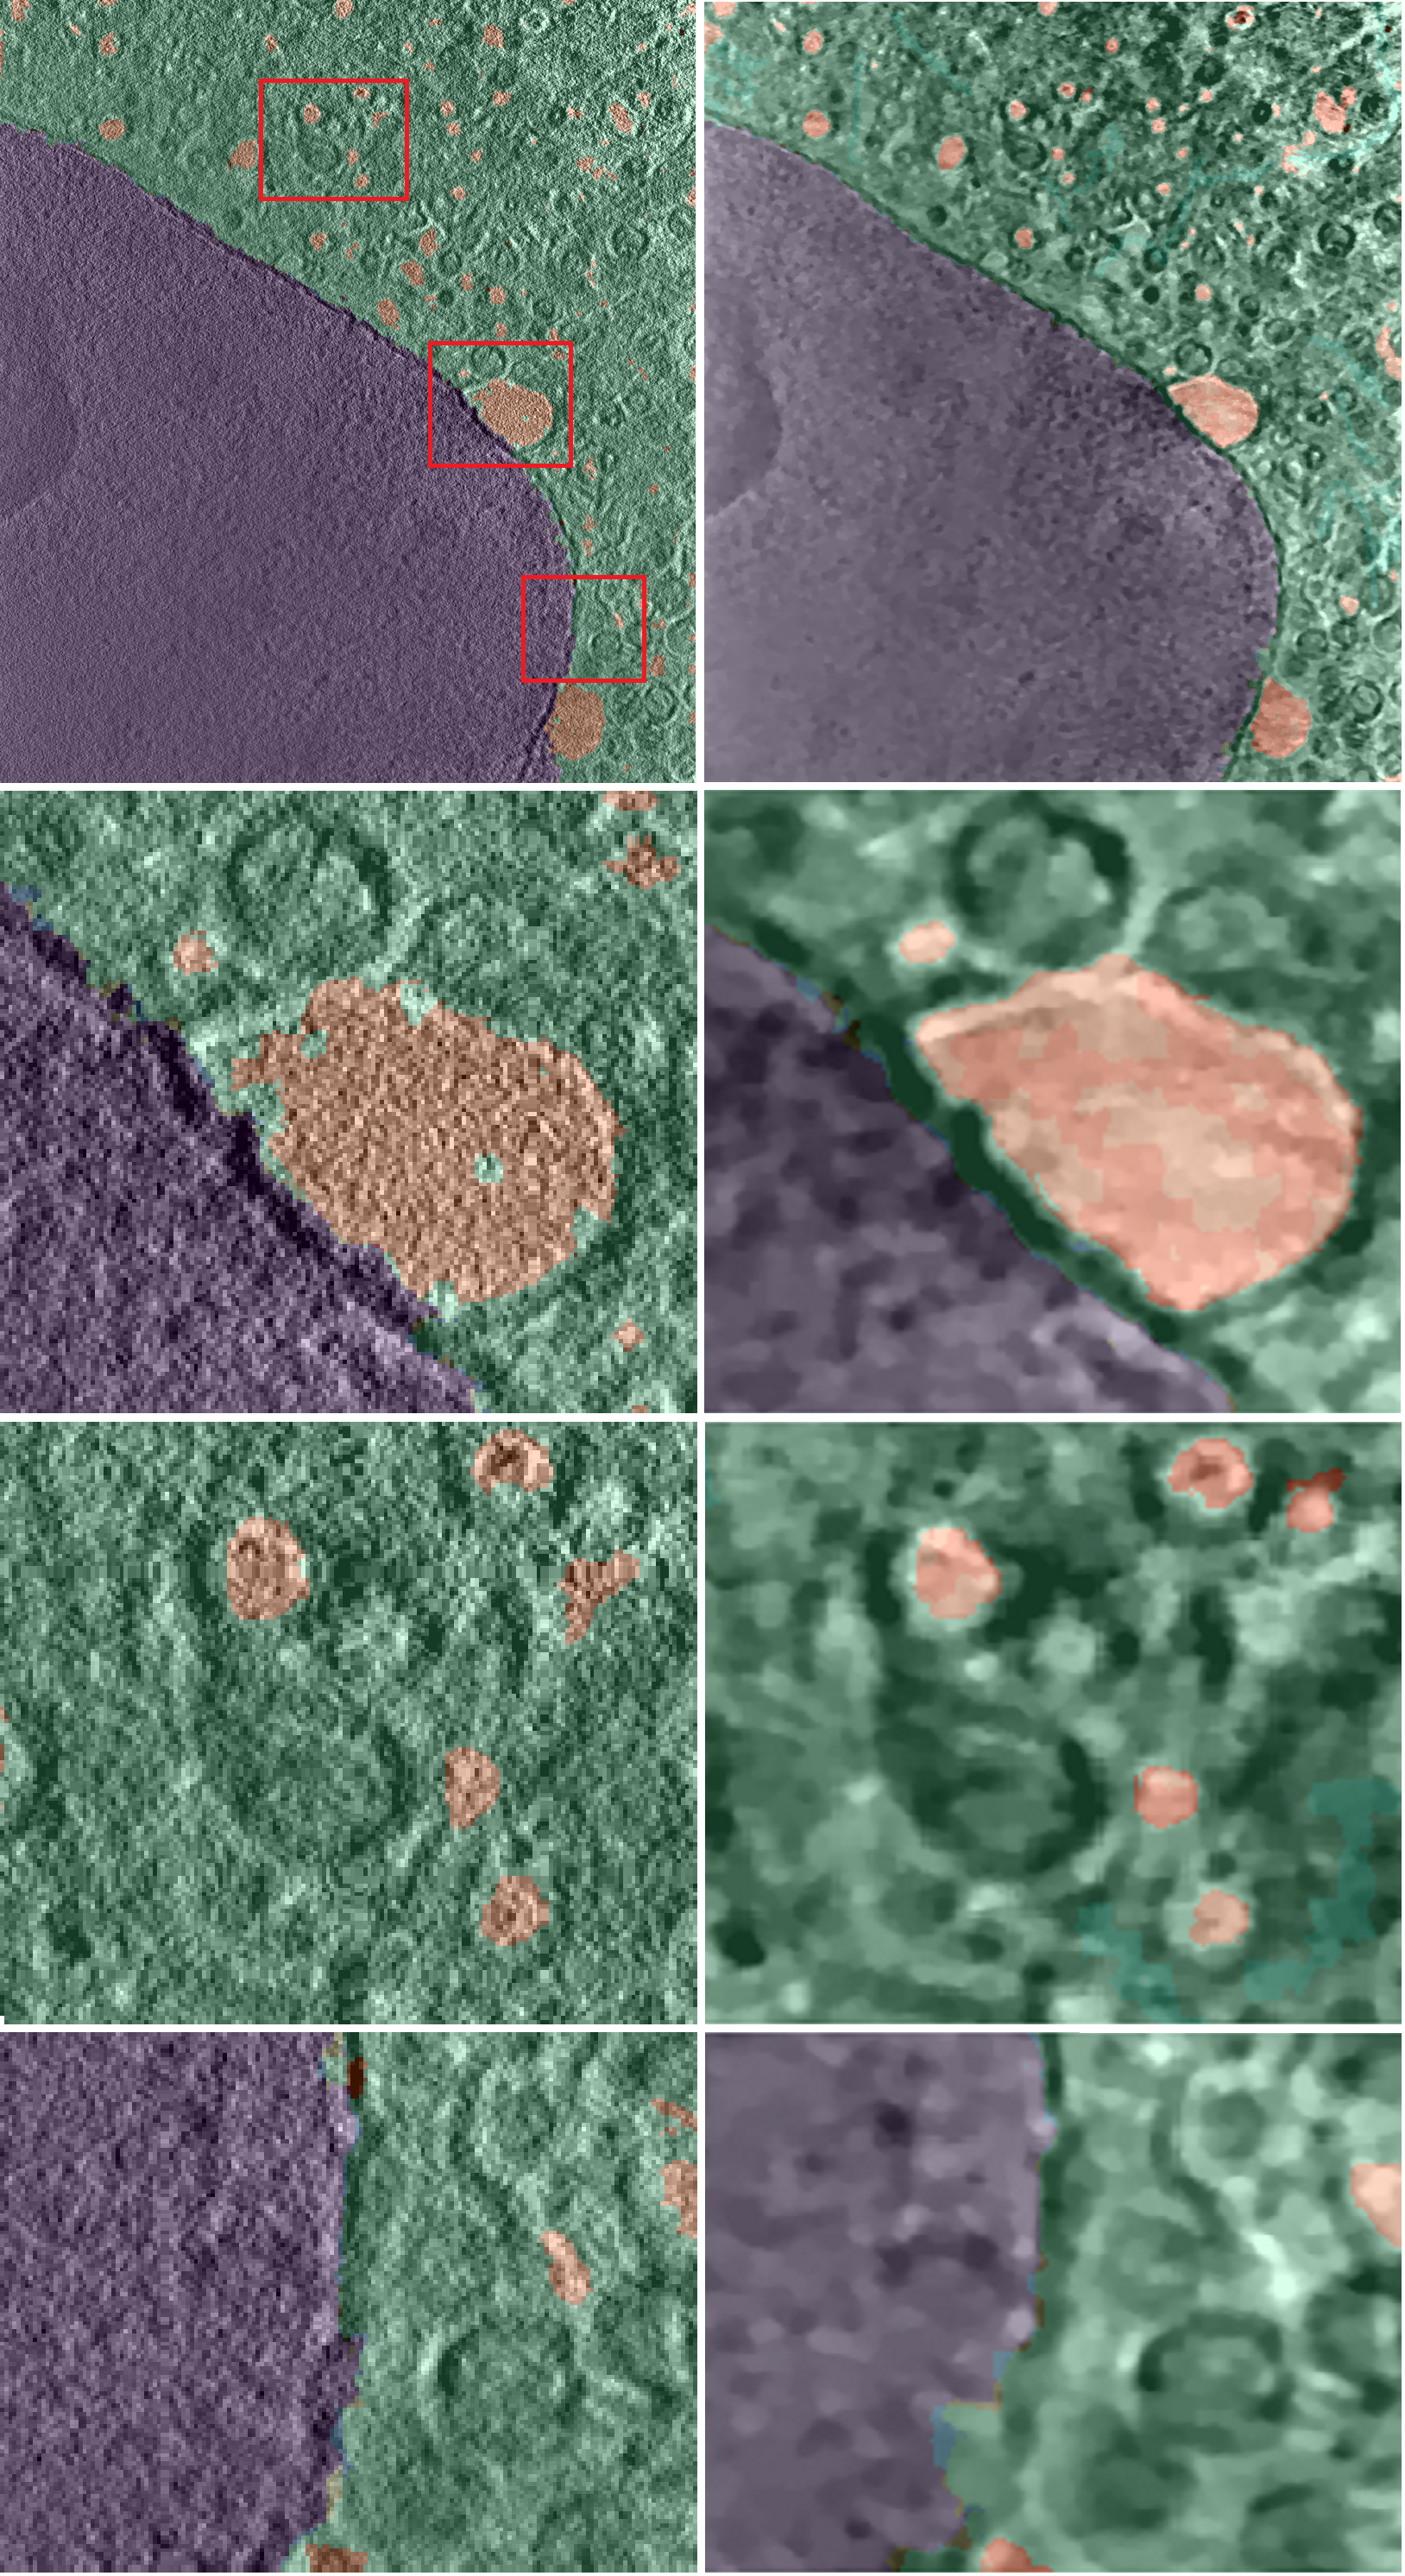
\includegraphics[height=0.8\textheight]{Applications/survos.png} 

\end{center}

\caption[Cell images segmented using SuRVoS for FBP and TV]{\label{fig:survos} Automatic segmentation using manual labels as training data using the SuRVoS workbench, for two different algorithms. Columns: FBP and OS-ASD-POCS (30 iterations, 10 TV iterations each). The zoomed areas are highlighted in the FBP image. The red squares in the first row show the location of the zoomed-in areas from the second third and fourth row. Colours show different labels chosen by the automatic segmentation.} 
\end{figure}
\FloatBarrier
\section{Discussion}
This chapter explores X-ray tomography experiments and showcases the reconstruction differences between iterative algorithms in TIGRE, for different geometries and tomography types. The first part of the chapter highlights the behaviour difference between some setting of the algorithms in TIGRE. The importance of algorithm and hyperparameter selection is hopefully stressed enough, so is the behaviour of the TV algorithms under parameter change. Some of the behaviour presented, especially the divergent behaviour, is not intrinsic to the mathematics used, but it happens due to the fast implementation of the methods on GPUs. This is an expected behaviour in most fast reconstruction methods, as it happens due to the mismatch between the projector and backprojector. Existing matched operations exists, but are slower, as generally they require projecting multiple times to compute the perfect adjoint. 

For the real datasets, note that no pre- or post-processing has been applied to the data, but for some minor amount for the Cryo-SXT. This is to highlight the effect of the algorithms in the final image, instead of data processing techniques. It is a challenge to evaluate the quality of iterative algorithms using real datasets. Here a few have been shown and different algorithms used on them. For all the datasets, the stronger robustness against noise that iterative algorithms have is clear. The tests with SuRVoS on the Cryo-SXT hint that TV algorithms can lead to a more robust image for automatic segmentation methods, however more test would be need to confirm or refute this claim. The clear step to evaluate the quality of iterative algorithms would be to perform the segmentation steps proposed in the SophiaBeads dataset. Unfortunately time limitations did not allow this test to be carried out for this thesis. 
